\documentclass[aspectratio=1610]{beamer}
\setbeamersize{text margin left=7mm,text margin right=5mm}
\usefonttheme[onlymath]{serif}
\usetheme{default}
\usefonttheme{professionalfonts}
%\setbeamertemplate{navigation symbols}{} 
\beamertemplatenavigationsymbolsempty
\addtobeamertemplate{navigation symbols}{}{
    \usebeamerfont{footline}
    \usebeamercolor[fg]{footline}
    %\hspace{1em}
    \footnotesize\insertframenumber\,%/\inserttotalframenumber
}

% cSpell:disable
\definecolor{rcomment}{rgb}{0.3, 0.3, 0.3}  % darkgrey
\definecolor{rred}{rgb}{0.7,0.2,0.2}        % red
\definecolor{rblue}{rgb}{0.2,0.2,0.7}       % blue (blended blue of beamer)
\definecolor{rpurple}{rgb}{0.45, 0.0, 0.9}  % violett
\definecolor{rpink}{rgb}{0.8, 0.0, 0.4}     % pink
\definecolor{rgreen}{rgb}{0.1, 0.5, 0.1}    % darkgreen
\definecolor{rorange}{rgb}{0.8, 0.4,0}      % orange
\definecolor{rblack}{rgb}{0, 0, 0}          % black
\definecolor{deeptuerkis}{rgb}{0, 0.5, 0.5} % Türkis
\definecolor{darkgreen}{rgb}{0,0.5,0}
\definecolor{blendedblue}{rgb}{0.2,0.2,0.7}
\newcommand{\important}[1]{{\color{green!60!black}#1}}

% \documentclass{beamer}
% \mode<presentation> {
%   \usetheme{Singapore}
%   \setbeamertemplate{navigation symbols}{}
%   \setbeamertemplate{footline}[frame number]
% }

\usepackage[utf8]{inputenc}
\usepackage{caption}
\usepackage{nicefrac}
\usepackage{varwidth}
\usepackage{amsmath}
\usepackage{hyperref}
\usepackage{color}
\usepackage{xcolor}
\usepackage{appendixnumberbeamer}
\usepackage{booktabs}
\usepackage{multirow}
\usepackage{siunitx}	% Allows to format numbers in tables
\usepackage{makecell}	% Allows line breaks in table text
\usepackage{multirow}	% Allows line breaks in table text
\usepackage{graphicx}
% \usepackage[table,xcdraw]{xcolor}
% Beamer presentation requires \usepackage{colortbl} instead of \usepackage[table,xcdraw]{xcolor}
\usepackage{colortbl}

\usepackage{pgfplots}
\pgfplotsset{compat=newest}
\usepgfplotslibrary{statistics}

\usepackage{tikz}
\usetikzlibrary{arrows,automata}
\usetikzlibrary{datavisualization}
\usetikzlibrary{positioning}
\usetikzlibrary{calc}
\usetikzlibrary{patterns}
\usetikzlibrary{matrix}
\usetikzlibrary{decorations.pathreplacing}
\usetikzlibrary{shapes.geometric, arrows, arrows.meta}

\tikzstyle{vertex} = [circle, draw=black, fill=black, minimum width=0.15cm, inner sep=0cm, text centered]
\tikzstyle{arc} = [thick,->,>=stealth]
\tikzstyle{emphvertex} = [circle, draw=red, fill=red, minimum width=0.15cm, inner sep=0cm, text centered]
\tikzstyle{empharc} = [thick,->,>=stealth, draw=red]
\tikzstyle{vertex-green} = [circle, draw=ForestGreen, fill=ForestGreen, minimum width=0.15cm, inner sep=0cm, text centered]
\tikzstyle{arc-green} = [very thick,->,>=stealth, draw=ForestGreen] %thick, very thick, ultra thick
\tikzstyle{bgvertex} = [circle, draw=black!40, fill=black!40, minimum width=0.15cm, inner sep=0cm, text centered]
\tikzstyle{bgarc} = [draw=black!40,thick,->,>=stealth]
\tikzstyle{move} = [thick, ->, -Implies, double,double distance=0.7mm]
\tikzstyle{cyclearc} = [thick,->,>=stealth,draw=red]
\tikzstyle{gets} = [thick, ->, -{Implies[length=5mm, width=3mm]}, double, double distance=1mm]

\usepackage{rotating}
\usepackage{subcaption}
\usepackage{cancel}

\newcommand\hcancel[2][black]{\setbox0=\hbox{$#2$}%
\rlap{\raisebox{.45\ht0}{\textcolor{#1}{\rule{\wd0}{1pt}}}}#2} 


% CHEATING DASH FROM https://tex.stackexchange.com/a/133357/128068
\tikzset{
	cheating dash/.code args={on #1 off #2}{
		% Use csname so catcode of @ doesn't have do be changed.
		\csname tikz@addoption\endcsname{%
			\pgfgetpath\currentpath%
			\pgfprocessround{\currentpath}{\currentpath}%
			\csname pgf@decorate@parsesoftpath\endcsname{\currentpath}{\currentpath}%
			\pgfmathparse{\csname pgf@decorate@totalpathlength\endcsname-#1}\let\rest=\pgfmathresult%
			\pgfmathparse{#1+#2}\let\onoff=\pgfmathresult%
			\pgfmathparse{max(floor(\rest/\onoff), 1)}\let\nfullonoff=\pgfmathresult%
			\pgfmathparse{max((\rest-\onoff*\nfullonoff)/\nfullonoff+#2, #2)}\let\offexpand=\pgfmathresult%
			\pgfsetdash{{#1}{\offexpand}}{0pt}}%
	}
}

\usepackage{mathtools}
%\usepackage{algorithm2e}
\usepackage[ruled,vlined]{algorithm2e} % Enables the writing of pseudo code.
\usepackage[draft,nomargin,inline]{fixme}
\usepackage{booktabs}

\usepackage[normalem]{ulem} % for strikethrough text
\newcommand\soutred{\bgroup\markoverwith{\textcolor{red}{\rule[0.5ex]{2pt}{0.4pt}}}\ULon} % for crossing out text in red

%******************************
%rest of frame
\usepackage{zref-savepos}

\newcounter{restofframe}
\newsavebox{\restofframebox}
\newlength{\mylowermargin}
\setlength{\mylowermargin}{2pt}

\newenvironment{restofframe}{%
	\par\centering
	\stepcounter{restofframe}%
	\zsavepos{restofframe-\arabic{restofframe}-begin}%
	\begin{lrbox}{\restofframebox}%
	}{%
\end{lrbox}%
\setkeys{Gin}{keepaspectratio}%
\raisebox{\dimexpr-\height+\ht\strutbox\relax}[0pt][0pt]{%
	\resizebox*{!}{\dimexpr\zposy{restofframe-\arabic{restofframe}-begin}sp-\zposy{restofframe-\arabic{restofframe}-end}sp-\mylowermargin\relax}%
	{\usebox{\restofframebox}}%
}%
\vskip0pt plus 1filll\relax
\mbox{\zsavepos{restofframe-\arabic{restofframe}-end}}%
\par
}

\let\oldfootnotesize\footnotesize
\renewcommand*{\footnotesize}{\oldfootnotesize\fontsize{6}{4}\selectfont}

% reset footnote counter for each frame
\AtBeginEnvironment{frame}{\setcounter{footnote}{0}}

% command for bold blue text
%\DeclareTextFontCommand{\structure}{\color{TuWienBlue}\bfseries}


%\usepackage{natbib}
% \usepackage[backend=bibtex,style=authoryear-comp]{biblatex}
% \bibliography{bibliography}
\usepackage[round]{natbib}
\bibliographystyle{plainnatnourl}


\usepackage[draft,nomargin,inline]{fixme}  % add final for disabling remarks
\fxsetface{inline}{\itshape}
\fxsetface{env}{\itshape}
%\fxuselayouts{margin}
%\fxuselayouts{inline}
\fxusetheme{color}

% \renewcommand{\thefootnote}{\fnsymbol{footnote}}
% cSpell:enable

\title{Scaling up Solving Approaches for Combinatorial Optimization\\ with Machine Learning}

\author{Günther R.\ Raidl}
\date{CDSAI Workshop on Evolutionary Machine Learning and Optimisation\\ Victoria University of Wellington, NZ\\July 12, 2024}
\titlegraphic{
\includegraphics[height=7mm]{graphics/logo-tuwien-informatics.png}\quad
	
\includegraphics[height=7mm]{graphics/AClongColor.pdf}}

\institute[]{\normalsize Algorithms and Complexity , TU Wien, Austria,\\
    \texttt{raidl@ac.tuwien.ac.at}\\[1ex]
}

\logo{
\includegraphics[height=15pt]{graphics/logo.pdf}\vspace{245pt}} % Logo on top right

% cSpell:disable
\definecolor{rred}{rgb}{0.7,0.2,0.2}         % red
\newcommand{\hl}[1]{\textcolor{rred}{#1}}    % highlight

\definecolor{rgreen}{rgb}{0.216,0.784,0.216} % green
\definecolor{rblue}{rgb}{0.216,0.443,0.784}  % blue
\definecolor{rorange}{rgb}{1.0,0.4,0.0}      % orange

\definecolor{orange}{RGB}{255,100,66}
\definecolor{seaborn0}{HTML}{1f77b4}
\definecolor{seaborn1}{HTML}{ff7f0e}
\definecolor{seaborn2}{HTML}{2ca02c}
\definecolor{seaborn3}{HTML}{d62728}
\definecolor{seaborn4}{HTML}{9467bd}
\definecolor{seaborn5}{HTML}{8c564b}
\definecolor{seaborn6}{HTML}{e377c2}
\definecolor{seaborn7}{HTML}{7f7f7f}
\definecolor{seaborn8}{HTML}{bcbd22}
\definecolor{seaborn9}{HTML}{17becf}

\newbool{printlegend}

\newcommand{\cumuldistr}[7]{ % Arguments: source directory, data series, width, height, x label, y label, title
  \begin{tikzpicture}
    \begin{semilogxaxis}[%
          width={#3},
          height={#4},
          title style={align=center},
          title={\large #7},
          xlabel style={at={(axis description cs:0.5,0.05)},anchor=north},
          xlabel=#5,
          ylabel style={align=center},
          ylabel=#6,
          every axis plot post/.append style={mark=none},
          every axis plot/.append style={thick},
          legend entries={GNN,Random,Sorted,Hooker},
          \ifbool{printlegend}{
            legend columns=1,
            legend pos=south east,
          }{
            legend to name=legend:cumuldistr-#1-#2,
            legend columns=-1,
          }
          ]
      \addplot+[seaborn0, solid]  table [x=#2, y=no_instances, col sep=comma, mark=none] {#1/pgdeletion_#2.csv};
      \addplot+[seaborn1, dashed] table [x=#2, y=no_instances, col sep=comma, mark=none] {#1/deletion_#2.csv};
      \addplot+[seaborn2, dashed] table [x=#2, y=no_instances, col sep=comma, mark=none] {#1/sdeletion_#2.csv};
      \addplot+[seaborn3, dashed] table [x=#2, y=no_instances, col sep=comma, mark=none] {#1/hdeletion_#2.csv};
    \end{semilogxaxis}
  \end{tikzpicture}
}
% cSpell:enable
\renewcommand{\footnotesize}{\scriptsize}


% ------------------------------------------------------------

\begin{document}{}


\part{Main}

\begin{frame}
  \titlepage
\end{frame} 


\section{Introduction}
%\subsection{Motivation}


\begin{frame}
	\frametitle{Motivation}
	\begin{minipage}{0.45\textwidth}
		\begin{center}
			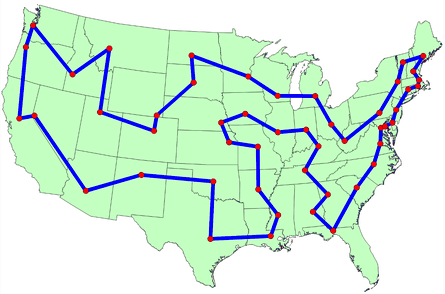
\includegraphics[width=0.9\textwidth]{graphics/48StatesTSP.png}

			\bigskip
			Algorithm \structure{MySuperTSPSolver}\\
			
\includegraphics[width=2cm]{graphics/hook.png}
		\end{center}
	\end{minipage}
	\qquad
	\frametitle{Motivation}
	\begin{minipage}{0.45\textwidth}
		\begin{center}
			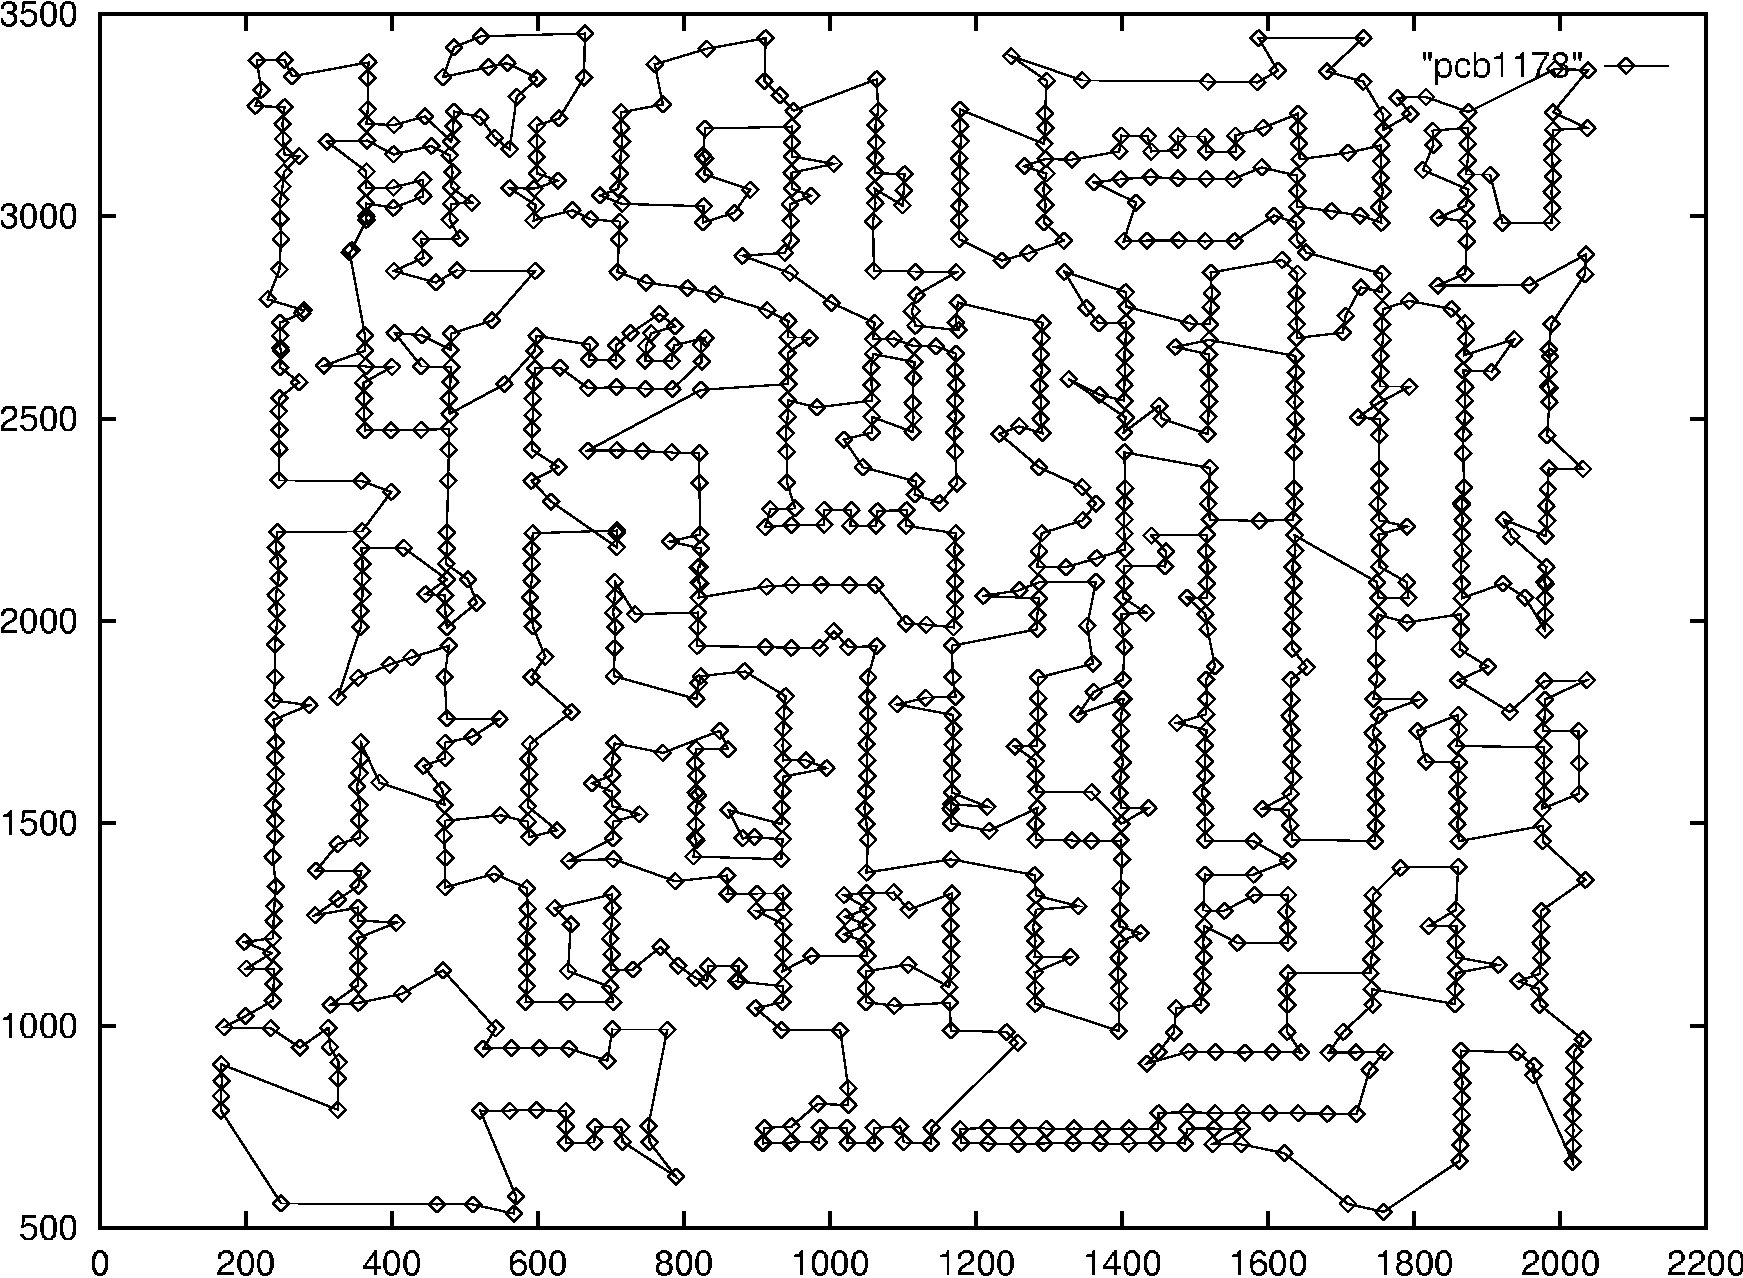
\includegraphics[width=0.9\textwidth]{graphics/TSPLeiter2opt.jpg}

			\bigskip
			\structure{MySuperTSPSolver} \alert{takes ``forever''}
			
\includegraphics[width=3cm]{graphics/question-mark.jpg}
		\end{center}
	\end{minipage}

\end{frame}

\begin{frame}{Motivation}

	\begin{center}
	\includegraphics<1>[width=0.4\textwidth]{graphics/hybrid-motivation.pdf}
	\includegraphics<2>[width=0.4\textwidth]{graphics/hybrid-motivation2.pdf}
	\end{center}

	\begin{itemize}
		\item 
		\structure{MySuperTSPSolver} does not scale well enough to (much) larger instances!
	
		\item \alert{Is different faster but cruder algorithm the only option?}
		\item<2> We aim at \important{\bf methods to improve the scalability} of MySuperTSPSolver,\\ (trading speed for quality).
	\end{itemize}
\end{frame}

\begin{frame}{Traditional/Naive Approaches}
	\begin{itemize}
	\item{\structure{Partition problem into smaller subproblems}\\
		solve them independently and combine solutions}\\
		\begin{center}
			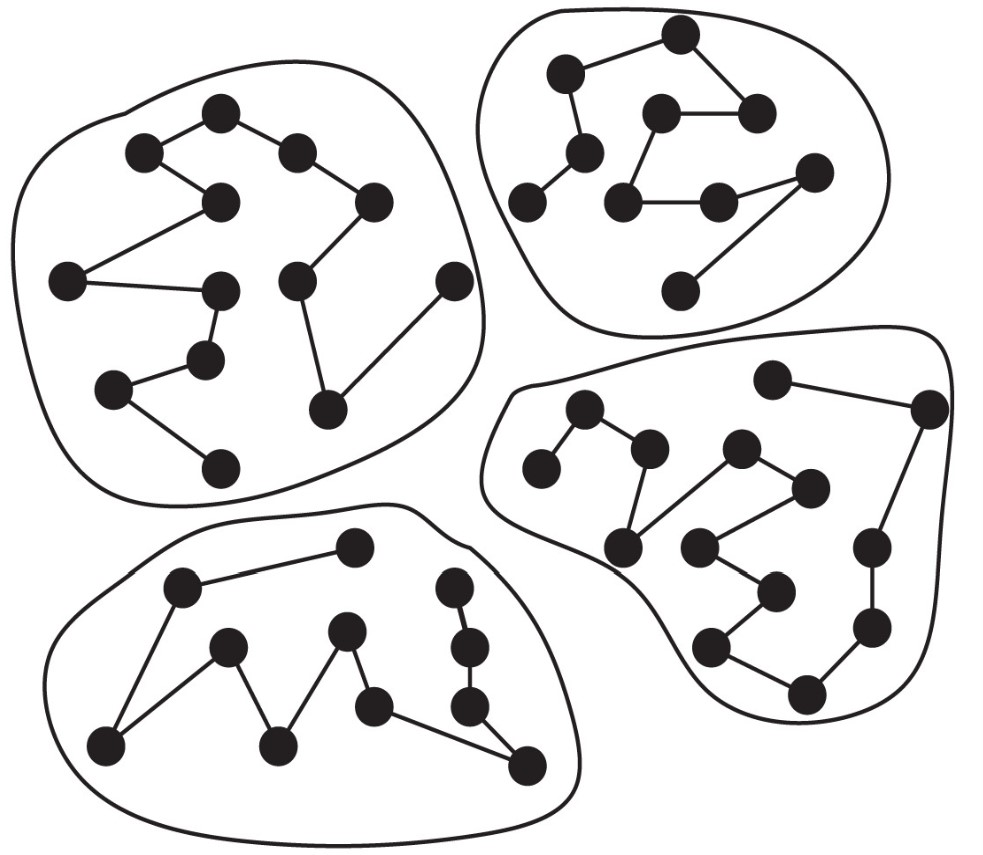
\includegraphics[width=0.22\textwidth]{graphics/partition.jpg}
		\end{center}
	\item<2>{\structure{Sparsifying the search space}}\\
		e.g., only consider $k$-nearest neighbor graph for TSP, VRP; \# edges: $O(n^2)\rightarrow O(n)$\\
		\begin{center}
			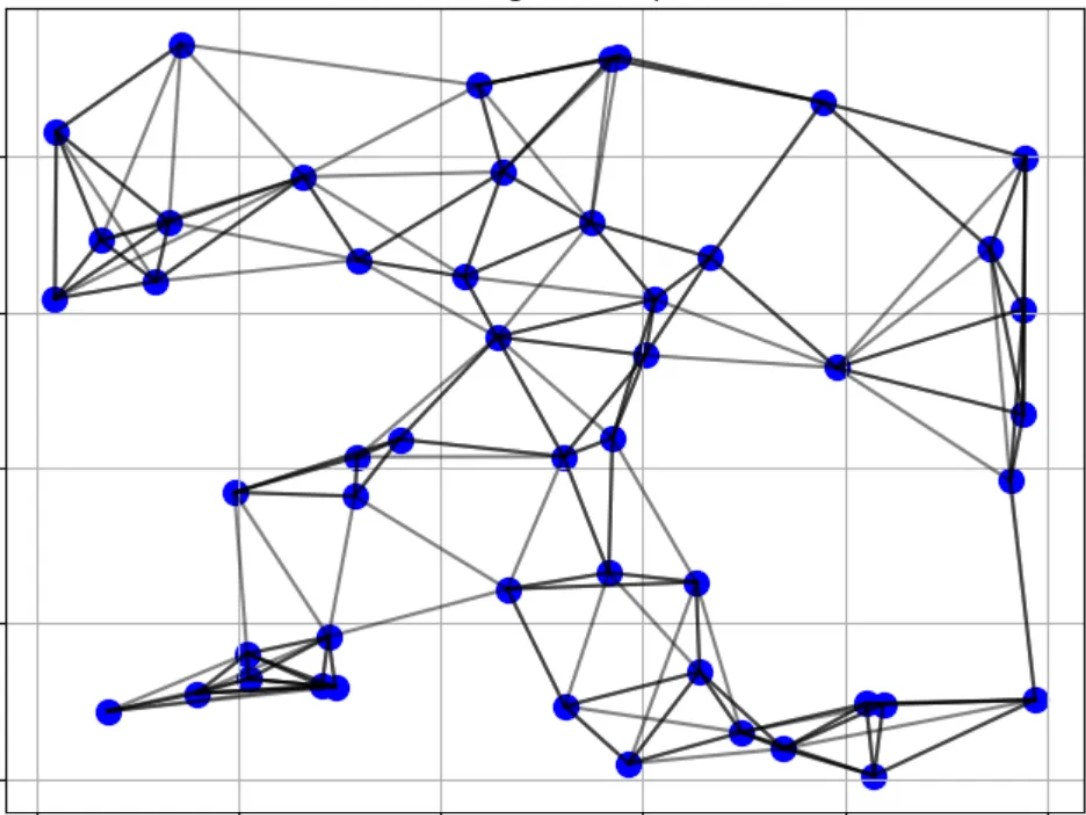
\includegraphics[width=0.28\textwidth]{graphics/kNN-graph.jpg}
		\end{center}
	\end{itemize}
\end{frame}

\begin{frame}{(Hybrid) Metaheuristic Approaches}
	\begin{itemize}
		\itemsep5ex
		\item \structure{Large Neighborhood Search (LNS)}\\
		\begin{itemize}
			\item Iteratively \important{destroy} parts of the solution by removing elements
			\item and \important{repair} it by solving the respective subproblem
			\item \alert{crucial:} choice of destroyed parts
		\end{itemize}
		\item \structure{Construct, Merge, Solve, and Adapt (CMSA)} \citep{blum-16b}
		\item \structure{POPMUSIC: Partial Optimization Metaheuristic Under Special Intensification Conditions} \citep{taillard-02}
		\item \ldots
	\end{itemize}
\end{frame}

\begin{frame}{Issues}
	While above strategies sometimes work well on academic problems,\\ they \alert{{\bf often fail} in more complex real-world scenarios}, e.g.,
	
	\bigskip
	\begin{itemize}
		\itemsep2ex
		\item because it is \alert{unclear which solution components are more or less promising}
		\item or \alert{more or less related to each other}. 
	\end{itemize}

	\vspace{1cm}
	\important{\bf Can we use machine learning for such aspects?}
	\begin{itemize}
		\item Focus here: offline, on representative training instances
	\end{itemize}
\end{frame}



\begin{frame}{A Multilevel Optimization Approach for
	Large Scale\\ Battery Exchange Station Location Planning}

Jatschka, Rodemann, and Raidl (EvoCOP, 2023) \cite{jatschka-23}

\medskip
from a joint project with Honda Japan and Honda Research Institute Europe

\bigskip
\begin{center}
	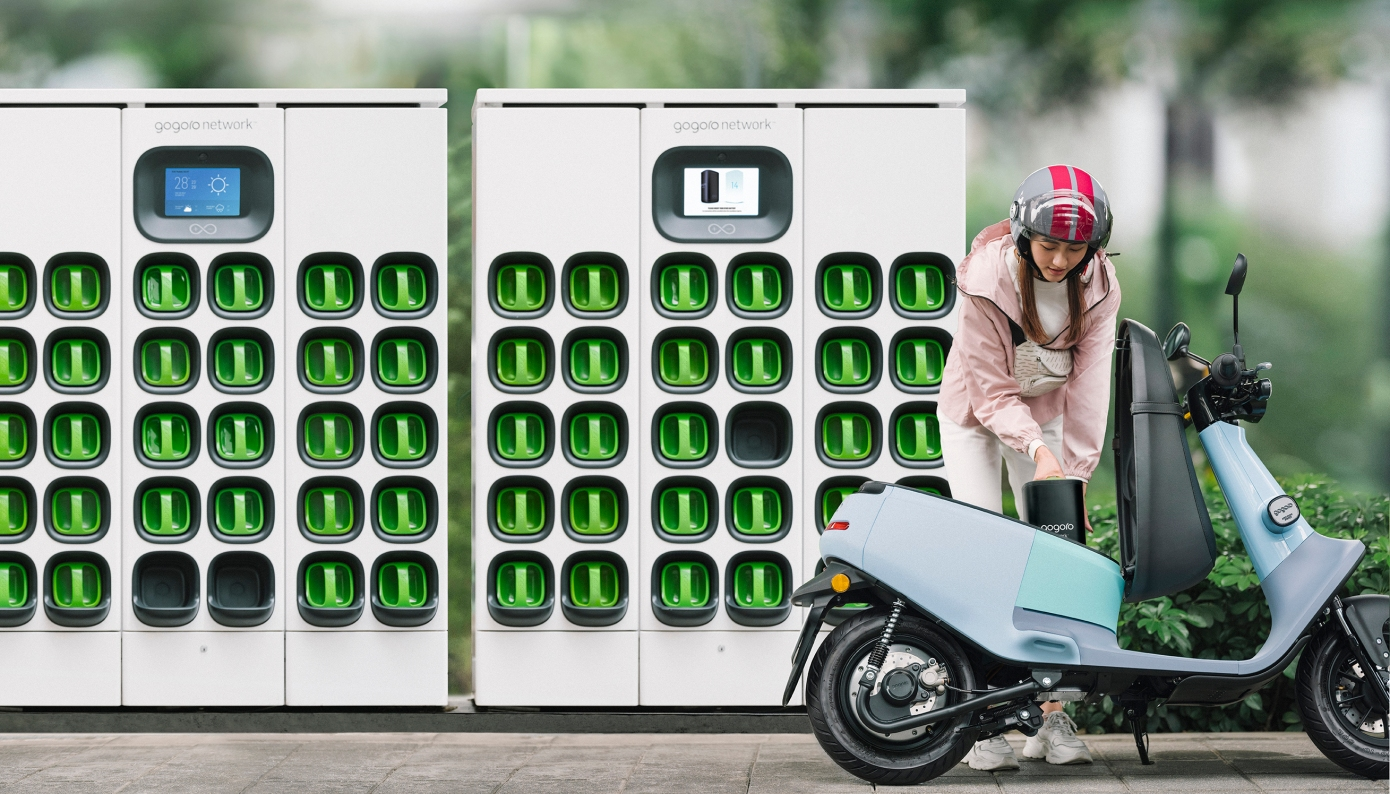
\includegraphics[width=0.6\textwidth]{graphics/Gogoro_Swapping_Station.jpg}\\
	{\small (c) Gogoro Inc.}
\end{center}
\end{frame}

\begin{frame}
\begin{itemize}
\item \structure{Given:} 
	\begin{itemize}
		\item Potential locations for battery exchange stations
		\item Origin/Destination (O/D) pairs of expected trips
	\end{itemize}
\item \structure{Goal:}
	\begin{itemize}
		\item Decide where to build stations with which capacities
		\item to maximize fulfilled demand while minimizing costs
	\end{itemize}
\end{itemize}

\begin{center}
	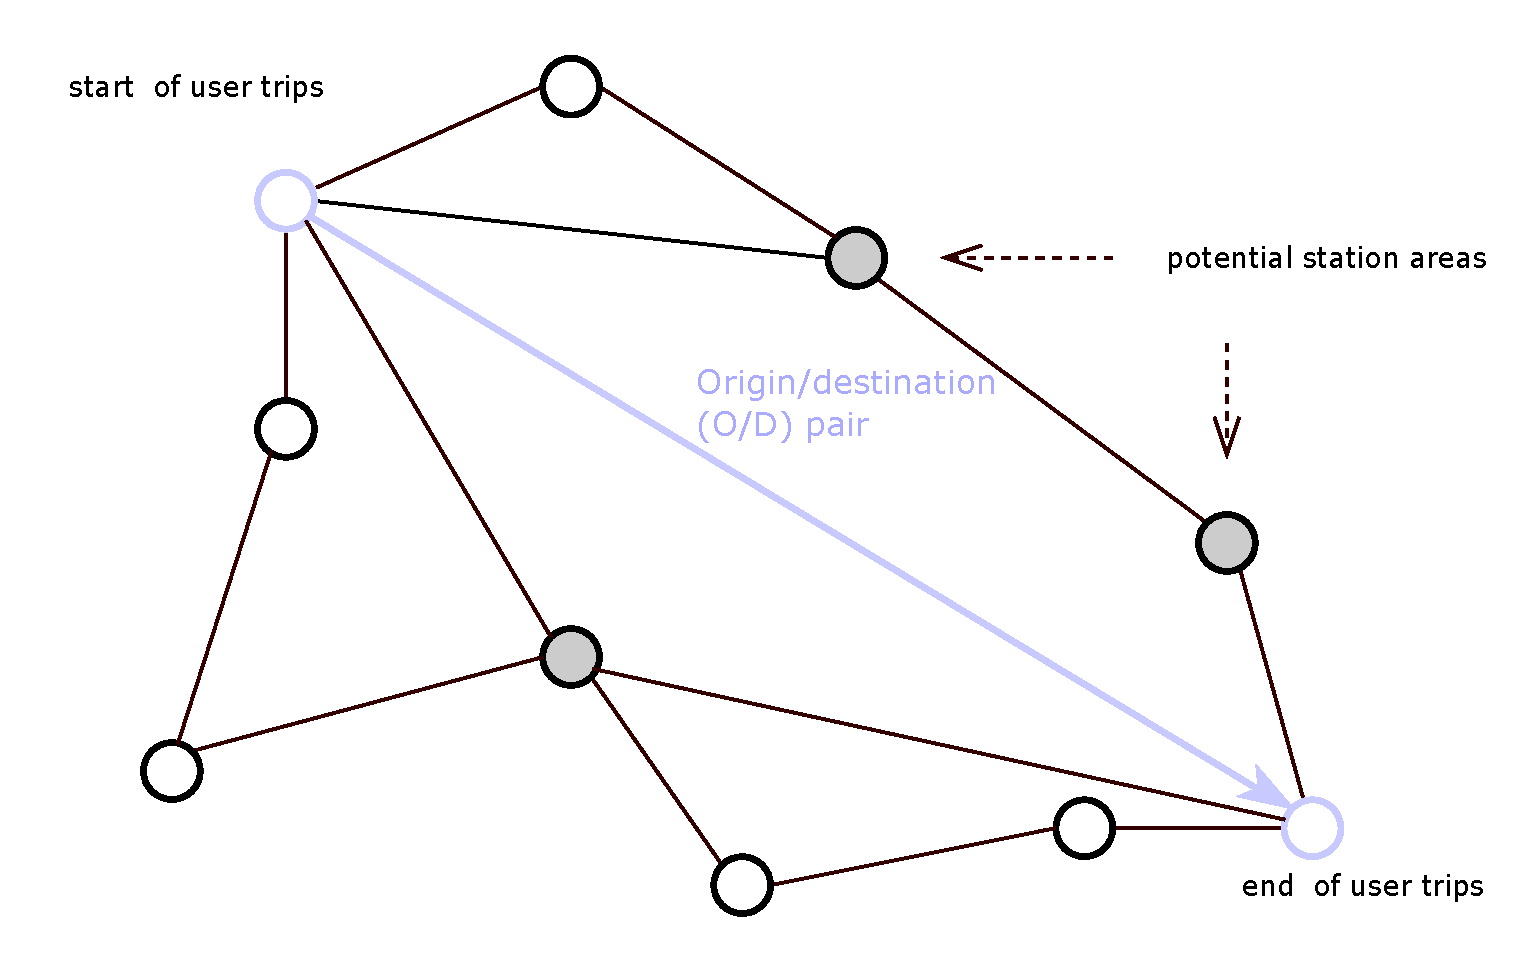
\includegraphics[width=0.6\textwidth]{graphics/graph_second.pdf}
	\includegraphics<2>[width=0.6\textwidth]{graphics/graph_third.pdf}
\end{center}
\end{frame}



% ### Bibliography ################################################################################

\begin{frame}[allowframebreaks]
	\frametitle{References}
	%\fontsize{6pt}{7.2}\selectfont
	\small
	\bibliography{lit}
\end{frame}



\end{document}





\end{document}
\begin{frame}{Multilevel Optimization}

	\footnotesize{\textcolor{gray}{\cite{walshaw-04}}}
	\begin{enumerate}
		\item \imp{\bf Coarsening:} contract edges\\ e.g., all edges
		belonging to a minimum weight maximal matching 
		
		\item Repeat (1) until threshold size is reached
		
		\item Solve partitioning problem on the coarsest graph
		
		\item \imp{\bf Extend and refine} solution to the next lower
		level\\ e.g., use Kernighan-Lin bisection algorithm
		
		\item Repeat (4) until solution to original graph is obtained
		
		\item Optional: iteratively \imp{\bf recoarsen} and extend+refine 
		%the graph\\ s.t.\ edges are only contracted within a subset
	   \end{enumerate}
	\begin{center}
		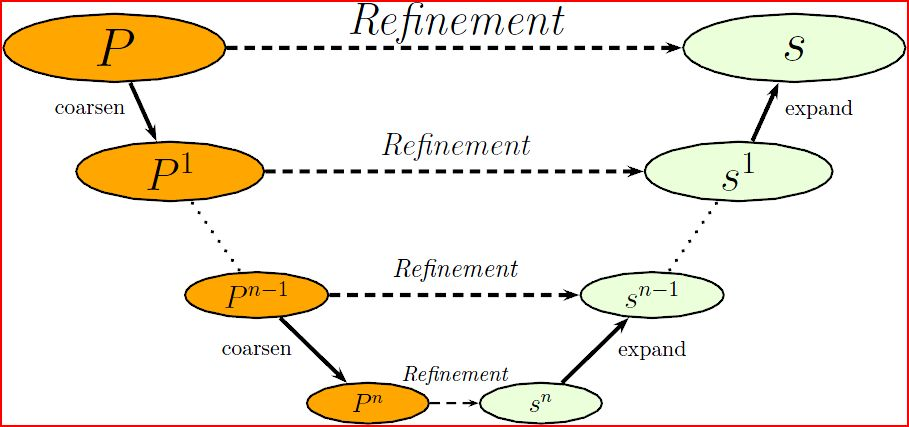
\includegraphics[width=0.6\textwidth]{graphics/multilevel.jpg}\\
		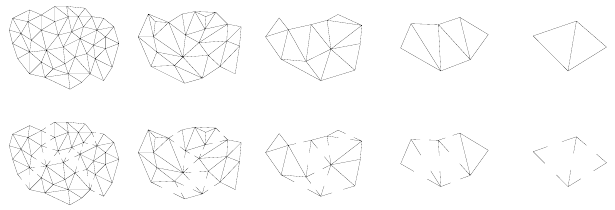
\includegraphics[width=0.6\textwidth]{graphics/mlr-gpp.png}
	\end{center}
\end{frame}\end{frame}

%old, shorter version
\begin{frame}
	\frametitle{Motivation}% \footnotesize{\textcolor{gray}{\cite{Ho:2018}}}}
	
\structure{Transportation services} 
\medskip
\begin{itemize}
	\item Classic public transit services (bus, train)
		\begin{itemize}
			\item[+] Many passengers, cost efficient
			\item[--] Fixed routes, scheduled times, unavailability
		\end{itemize}
	\smallskip
	\item Taxi services 
		\begin{itemize}
			\item[+] Door-to-door service 
			\item[--] High cost
		\end{itemize}
	\smallskip
	\item On-demand public transit services = \important{\bf Dial-A-Ride (DAR)}
		\begin{itemize}
			\item[+] Cost efficient, environment-friendlier, customizable service
			\item[--] Ride-sharing, detours
		\end{itemize}
\end{itemize}
	
\end{frame}

\end{document}

\begin{frame}
	\frametitle{Dial-A-Ride Problem (DARP) \footnotesize{\textcolor{gray}{\cite{Cordeau:2003}}}}

\onslide<1->{
\begin{minipage}{0.47\textwidth}
\begin{itemize}
	\item Combinatorial optimization problem
	\item NP-hard
	\item Generalization of: 
		\begin{itemize}
			\item Capacitated vehicle routing problem
			\item Pickup and delivery problem 
		\end{itemize}
\end{itemize}
\end{minipage}
\hfill
\begin{minipage}{0.47\textwidth}
\begin{figure}
	\centering
	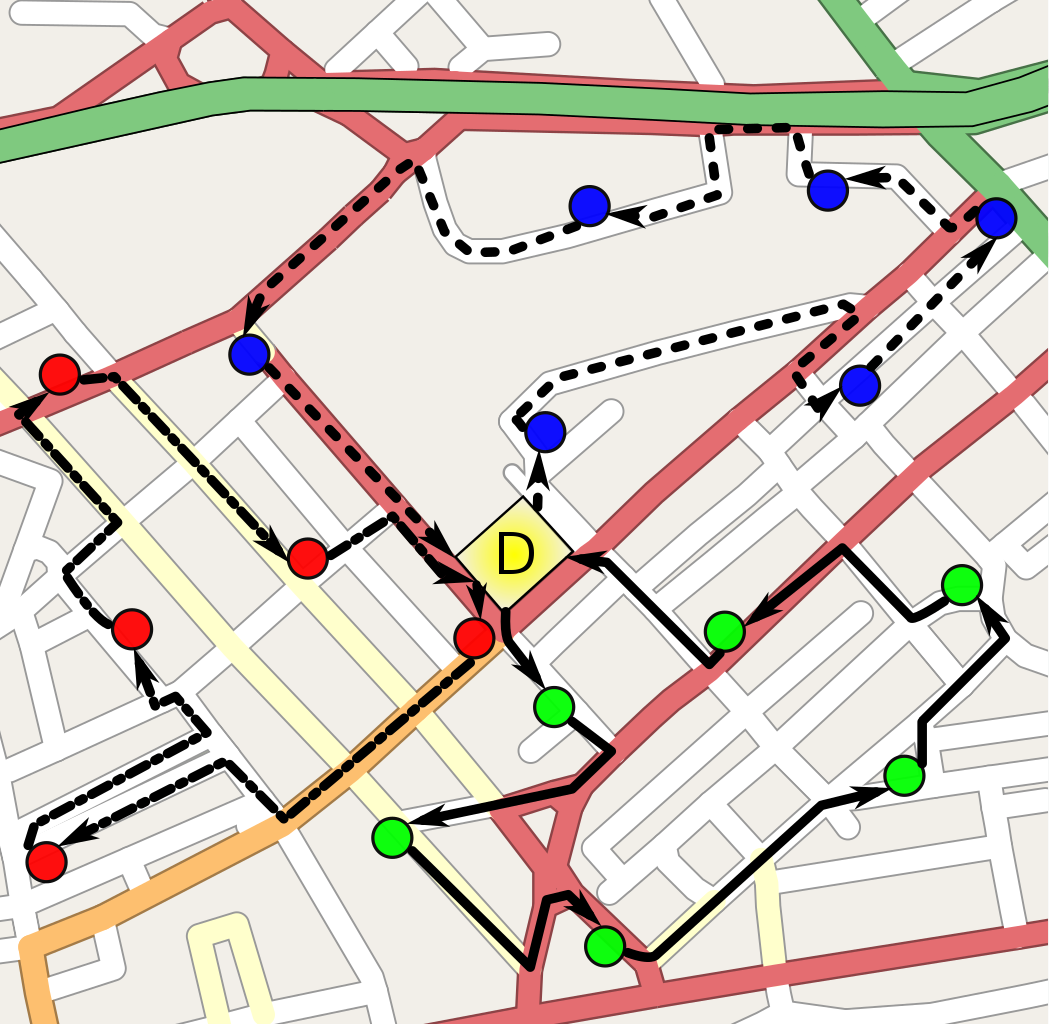
\includegraphics[width=0.6\textwidth]{graphics/sdd-example.png}
	%\caption{Free to use, CC license?.}
\end{figure}
\end{minipage}
}

\begin{definition}[\textsc{Dial-A-Ride Problem}]
    \structure{Given:}\\ $n$ users with transportation \important{requests} from a pickup to a drop-off location,\\ a \important{fleet} of $m$ vehicles

	\medskip
    \structure{Task:}\\ Find \important{routes} for $m$ vehicles serving all requests,\\ s.t.\ the \important{total routing cost} is minimized and certain constraints are satisfied.
\end{definition}
	
\end{frame}


% alternative2: too much text => keywords only 
% => show constraints one by one so there is not so much text to read at once
%(done) remove second part of second constraint, remove third constraint 
\begin{frame}
	\frametitle{DARP Constraints \footnotesize{\textcolor{gray}{\cite{Cordeau:2003}}}}
	
\begin{itemize}
	\itemsep2ex
	%[<important@+>] %important each bullet point on each slide -> problem with nested itemize; instead use important for each item to limit it to one slide in the frame 
%	\onslide<1->{\item<important@1> Every route starts and ends at the depot.}
	\item Start and end of each route at the depot
%	\onslide<2->{\item<important@2> For every request, the pickup and drop-off location belong to the same route and the drop-off is visited after the pickup location.} 
	\item Pickup and drop-off of request in same route 
%	\onslide<3->{\item<important@3> The load of a vehicle does not exceed the vehicle capacity at any time.} 
%	\onslide<4->{\item<important@4> The total duration of a route does not exceed the maximum route duration.} 
	\item Total route duration $\leq$ maximum route duration
%	\onslide<5->{\item<important@5> The service at each location begins in the given time window, and every vehicle leaves the depot and returns to the depot within the planning horizon.} 
	\item Each service starts within time window
%	\onslide<6->{\item<important@6> The ride time of any user does not exceed the maximum ride time. 
	\item User ride time $\leq$ maximum ride time 
		\begin{itemize}
			\item[$\color{red}{\rightarrow}$] consideration of user inconvenience %arrow is not colored by important, has to be done manually 
		\end{itemize}
\end{itemize}
	
\end{frame}


%\subsection{Electric Autonomous DARP (E-ADARP)}

\begin{frame}
	\frametitle{Electric Autonomous DARP (E-ADARP) \\ \footnotesize{\textcolor{gray}{\cite{Bongiovanni:2019}}}}
	
\begin{definition}[\textsc{Electric Autonomous DARP}]
    \structure{Given:} $n$ users with transportation requests from a pickup to a drop-off location,\\ a fleet of $m$ \important{electric autonomous} vehicles 

	\medskip
    \structure{Task:} Design $m$ vehicle routes serving all requests, s.t.\ the \important{total travel time and\\ the \textbf{excess ride times}} of all users are minimized and certain constraints are satisfied.
  \end{definition}
  
\begin{figure}
	\centering
	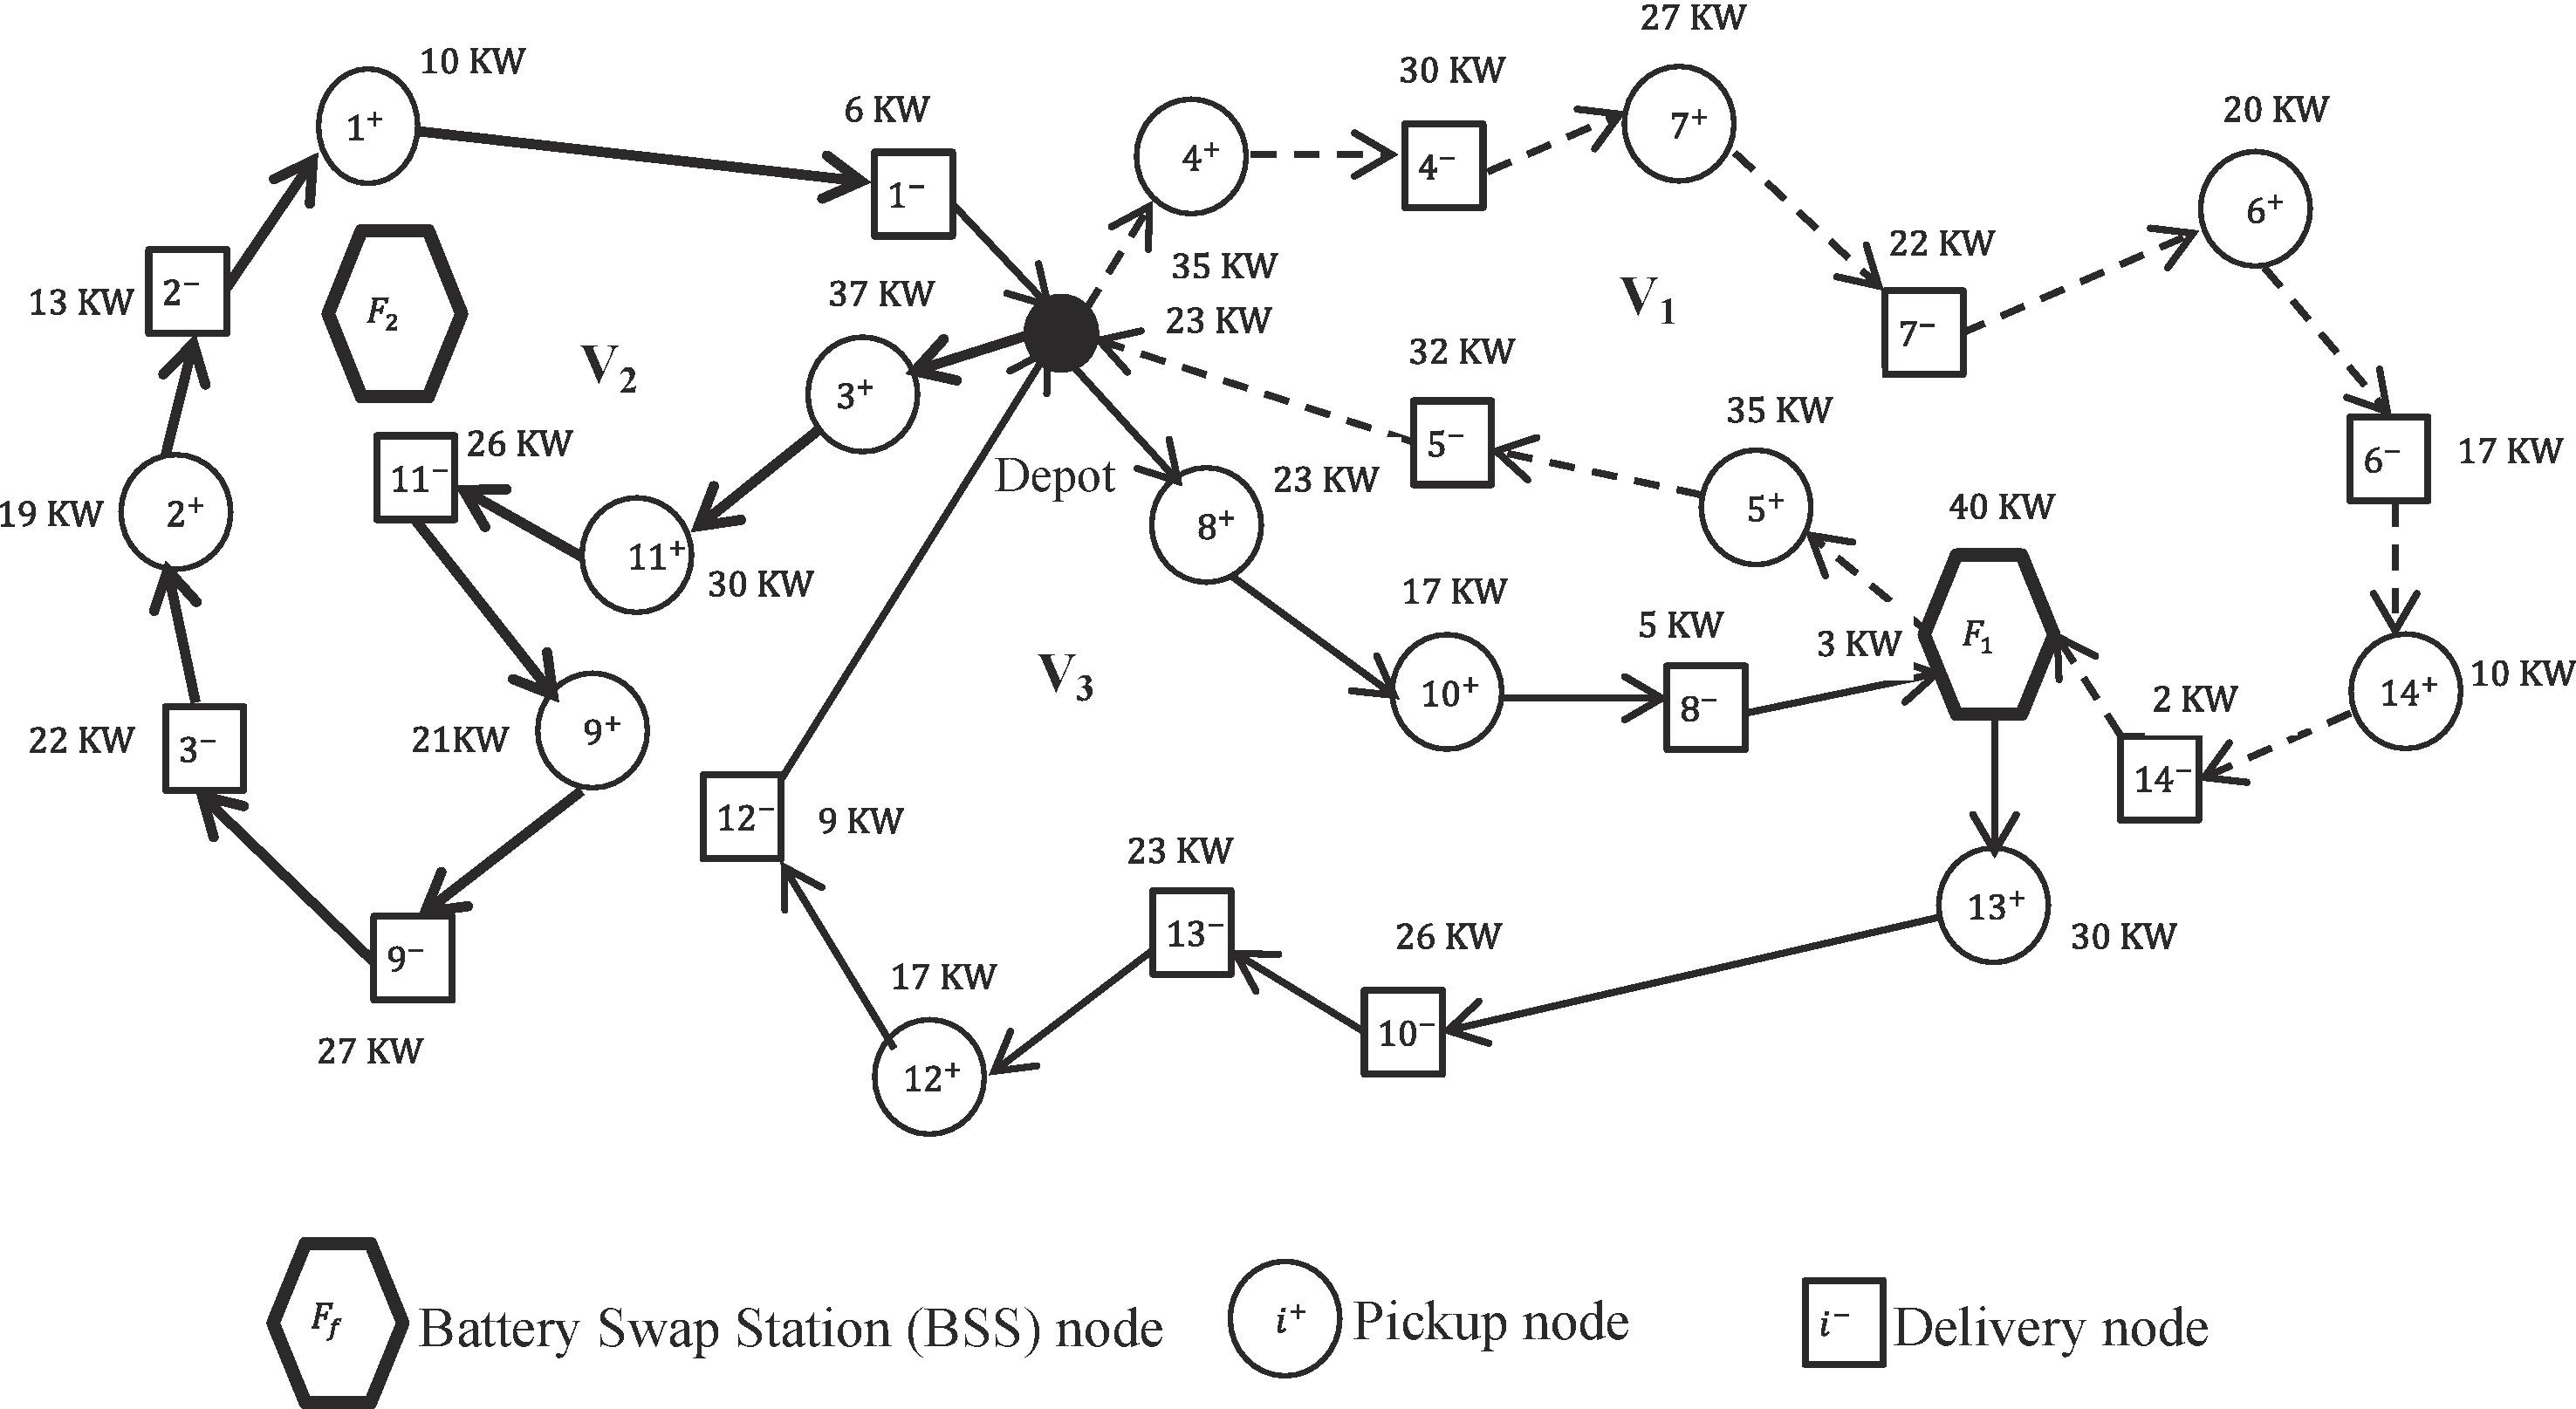
\includegraphics[scale=0.80]{graphics/darp-bss-example.jpg}
	%\caption{Example for E-DARP from \cite{Masmoudi:2018}.}
\end{figure}
	
\end{frame}

% new version to comply with new version for DARP constraints 
\begin{frame}
	\frametitle{E-ADARP Constraints \footnotesize{\textcolor{gray}{\cite{Bongiovanni:2019}}}}

\begin{itemize}
	\item Start and end at \soutred{the depot} $\rightarrow$ \important{one of multiple depots}
	\item Pickup and drop-off of request in same route
	\item \soutred{Total route duration $\leq$ maximum route duration}  
	\item Service starts within time window, vehicles leave and return to depot within planning horizon 
	\item User ride time $\leq$ maximum ride time 
		\begin{itemize}
			\item[$\rightarrow$] consideration of user inconvenience 
		\end{itemize}
\end{itemize}
	
\onslide<2>{
\textbf{\important{New constraints concerning battery management}} 
\begin{itemize}
%	\item The battery level of vehicles cannot exceed the battery capacity and cannot fall below zero at any time.
%	\item Vehicles have to return with minimal battery levels to the destination depots.
	\item Minimum battery levels when arriving at destination depots
%	\item Charging stations can only be visited when there is no user on board.
	\item Only vehicles without customers may charge 
%	\item Each charging station can only be visited at most once by all vehicles.
	\item At most one visit per charging station over all vehicles 
\end{itemize}

\bigskip
\structure{Simplifying assumptions:}
\begin{itemize}
	\item Constant battery consumption independent from load, speed, and SOC
	\item Constant charging rate 
\end{itemize}
}
\end{frame}


\section{Related Work}

\begin{frame}
  \frametitle{Related Work}
  	
\structure{Static E-ADARP:}
\medskip
\begin{itemize}
	\item Mixed integer linear programming (MILP) formulations and branch-and-cut algorithm by \cite{Bongiovanni:2019} 
		\begin{itemize}
			\item 2-index formulation e-ADARP2 
		\end{itemize}
	\smallskip
	\item Deterministic annealing (DA) algorithm by \cite{Su:2023}
		\begin{itemize}
			\item Linear-time exact route evaluation scheme % based on forward labeling % algorithm 
			%\item Battery-restricted fragments 
		\end{itemize}
	\smallskip
	\item Bilevel large neighborhood search (BI-LNS) by \cite{Limmer:2023}
		\begin{itemize}
%			\item Outer level: set/optimize visits to charging stations 
%			\item Inner level: insert/optimize requests 
			\item Outer level: charging stops 
			\item Inner level: requests 
		\end{itemize}
\end{itemize}

\bigskip

\structure{Dynamic E-ADARP:} %TODO maybe remove dynamic E-ADARP?
\medskip
\begin{itemize}
%	\item Machine learning-based 2-phase metaheuristic (ML-LNS) by \cite{Bongiovanni:2022}
	\item 2-phase metaheuristic by \cite{Bongiovanni:2022}
% 		\begin{itemize}
% %			\item First phase: greedy insertion heuristic
% %			\item Second phase: machine learning-based LNS 
% 			\item Machine learning-based LNS
% 		\end{itemize}
\end{itemize}
  
\end{frame}

%TODO use alternative 1, remove others
% alternative 1: 
\begin{frame}
  \frametitle{Battery-Restricted Fragments} %{\footnotesize{\textcolor{gray}{(\cite{Su:2023})}}}}
  
\begin{definition}[\textsc{Battery-restricted fragment}]
	A \important{\emph{battery-restricted fragment}}~$\mathcal{F} = (i_1, i_2, \dots, i_k)$ is a subsequence of a feasible route that consists only of \important{pickup and drop-off nodes}, where the vehicle \important{arrives empty} at $i_1$ and \important{leaves empty} at $i_k$ and has passenger(s) on board at all other nodes.
\end{definition}

% insert example of route with fragments (instead of first bullet point) -> e.g. from Su et al.
\begin{figure}
	\centering
	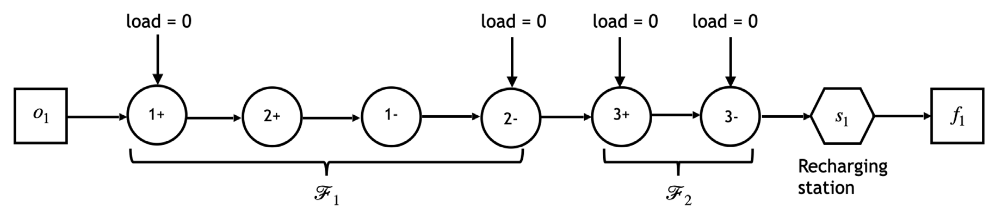
\includegraphics[scale=0.42]{graphics/battery-restricted-fragment-example.png}
	%\caption{Route with battery-restricted fragments, taken from \cite{Su:2023}.}
\end{figure}

\begin{itemize}
%	\item Route = concatenation of an origin depot, battery-restricted fragments, optional charging stations, and a destination depot 
%	\item Minimum user excess ride time $t^{\mathrm{excess}}_{\mathrm{min}}(\mathcal{F})$ of a fragment $\mathcal{F}$: calculated exactly with a linear program (LP)
	\item Charging within a fragment not allowed
	\item Timing within can be \important{independently optimized} to \important{minimize user excess ride time}\\ %$t^{\mathrm{excess}}_{\mathrm{min}}(\mathcal{F})$}\\
	$\rightarrow$ exactly determined by solving a \important{linear program (LP)}
	\item Fragments + results are \important{cached} to avoid repeated calculation
\end{itemize}

\end{frame}


% \begin{frame}
%   \frametitle{Battery-Restricted Fragments {\footnotesize{\textcolor{gray}{(\cite{Su:2023})}}}}
%   \framesubtitle{Usage}
  
% \structure{Efficient route cost computation:}
% \begin{itemize}
% 	\item Minimum user excess ride time of a feasible route $r$ with fragments $\mathcal{F}_1, \mathcal{F}_2, \dots, \mathcal{F}_n$: $t^{\mathrm{excess}}_{\mathrm{min}}(r) = \sum_{i = 1}^{n} t^{\mathrm{excess}}_{\mathrm{min}}(\mathcal{F}_i)$ 
% \end{itemize}

% \medskip
  
% \structure{\cite{Su:2023}:}
% \begin{itemize}
% 	\item Enumerate and evaluate all feasible fragments during preprocessing 
% 		\begin{itemize}
% 			\item[$\rightarrow$] can be inefficient, time-consuming, memory demanding 
% 		\end{itemize}
% %	\item Use precalculated user excess rides times during route evaluation
% \end{itemize}

% \medskip

% \structure{Our approach:}
% \begin{itemize}
% 	\item Evaluate fragments on first encounter 
% 		\begin{itemize}
% %			\item[$\rightarrow$] cache in hash table 
% 			\item[$\rightarrow$] better scalability 
% 		\end{itemize}
% 	\item Improve charging stop insertion %: used to improve efficiency as charging stations can only be inserted in between fragments and not within them 
% \end{itemize}

% \end{frame}


\section{Solving Approach}

%(done) preprocessing could be removed if presentation too long -> moved to additional slides 


\begin{frame}[noframenumbering]
	\frametitle{Large Neighborhood Search (LNS) \\ \footnotesize{\textcolor{gray}{\cite{Shaw:1998, Pisinger:2010}}}}

\begin{itemize}
	\item Based on
		\begin{itemize}
			\item (set of) destroy operator(s)
			\item (set of) repair operator(s)
		\end{itemize}
	%\item Important parameter: \important{degree of destruction~$k$}
\end{itemize}

\medskip
% pseudo code for LNS
\scalebox{0.8}{
\begin{algorithm}[H]
	\SetAlgoSkip{}
	\SetArgSty{textnormal}	% prints termination criterion in normal text instead of italics
	\SetKwFunction{FMain}{LNS}
	\SetKwProg{Fn}{Procedure}{:}{end}
	\KwIn{feasible solution $x$}
 	\KwOut{best found solution $x^b$}
	%\Fn{\FMain{}}{ % prints "Procedure LNS():"
  		%\Begin{
  			$x^b \leftarrow x$\;
			Select a destroy and a repair operator pair $(d,r)$\;
  			\Repeat{stop criterion is met}{
  				$x^t \leftarrow r(d(x))$\;
  				\If{$\text{accept}(x^t,x)$}{
  					$x \leftarrow x^t$\;
  				}
  				\If{$c(x^t) < c(x^b)$}{
  					$x^b \leftarrow x^t$\;
  				}
  			}
  			\Return{$x^b$\;}
  		%}
  	%}
  %\caption{Large Neighborhood Search procedure \texttt{LNS()} for a minimization problem}
  \caption{Large Neighborhood Search}
  \label{alg:large-neighborhood-search} % \label has to be placed AFTER \caption to produce correct cross-references.
\end{algorithm} 
}

% \onslide<3>{
% % example
% \begin{minipage}[t]{0.3\linewidth}
% \begin{figure}
% 	\centering
% 	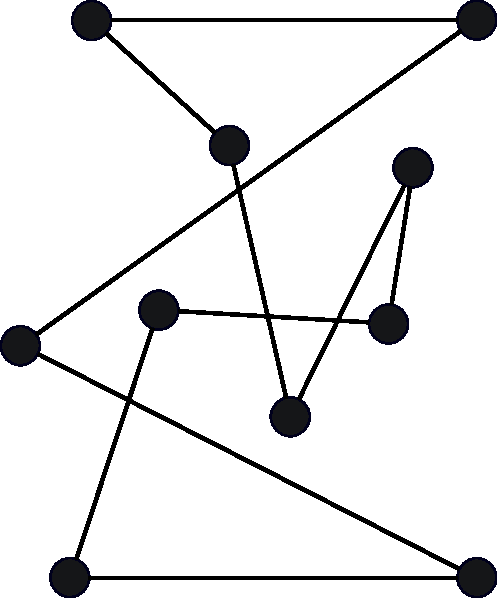
\includegraphics[width=\textwidth]{graphics/tsp-initial-solution}
% 	\caption{Initial solution.}
% \end{figure}
% \end{minipage}%
% \hfill%
% \begin{minipage}[t]{.3\textwidth}
% \begin{figure}
% 	\centering
% 	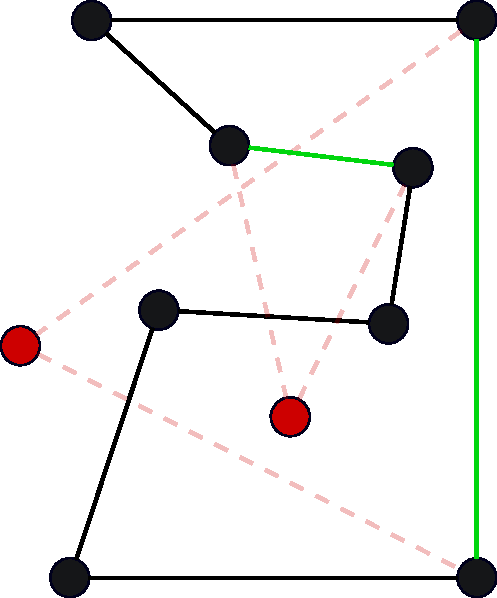
\includegraphics[width=\textwidth]{graphics/tsp-destroy-solution} 
% 	\captionof{figure}[]{After destroy operation.}
% \end{figure}
% \end{minipage}%
% \hfill%
% \begin{minipage}[t]{.3\textwidth}
% \begin{figure}
% 	\centering
% 	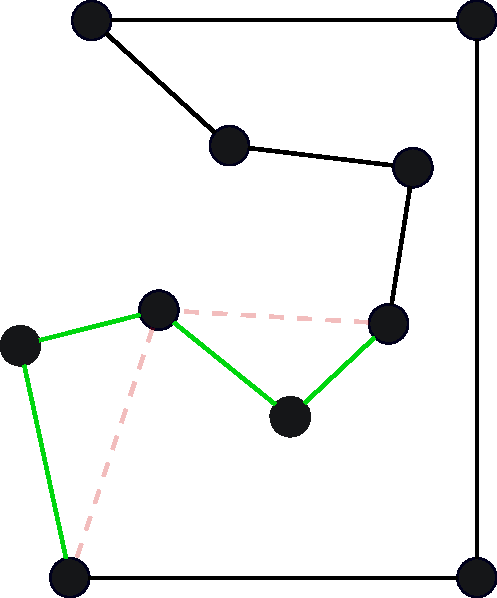
\includegraphics[width=\textwidth]{graphics/tsp-repair-solution} 
% 	\captionof{figure}[]{After repair operation.}
% \end{figure}
% \end{minipage}%
% }

\end{frame}


\subsection{Large Neighborhood Search (LNS)}

%(done) initial solution construction could be removed if presentation too long -> moved to additional slides

% destroy operator, repair operator
\begin{frame}
  \frametitle{Large Neighborhood Search (LNS)}

  Basic framework similar to {\textcolor{gray}{(\cite{Ropke:2006})}}
%  \framesubtitle{Destroy Operator}

%TODO insert figure of destroy operator or destroy-repair in LNS
% old figure
%\begin{minipage}[t]{\linewidth}
%\begin{figure}
%	\centering
%	\includegraphics[width=\textwidth]{graphics/lns-example-placeholder}
%	\caption{Initial solution (left), destroyed solution (middle), repaired solution (right).}
%\end{figure}
%\end{minipage}%
% new figures
%\begin{minipage}[t]{0.3\linewidth}
%\begin{figure}
%	\centering
%	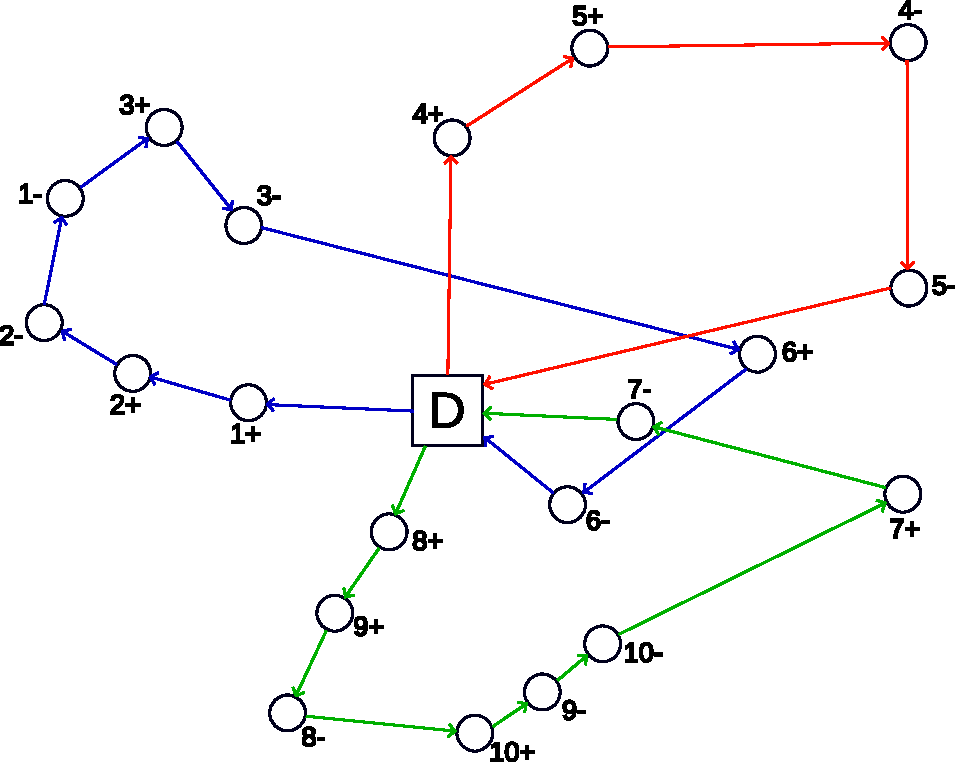
\includegraphics[width=\textwidth]{graphics/lns-initial-solution}
%	\caption{Initial solution.}
%\end{figure}
%\end{minipage}%
%\hfill%
%\begin{minipage}[t]{.3\textwidth}
%\begin{figure}
%	\centering
%	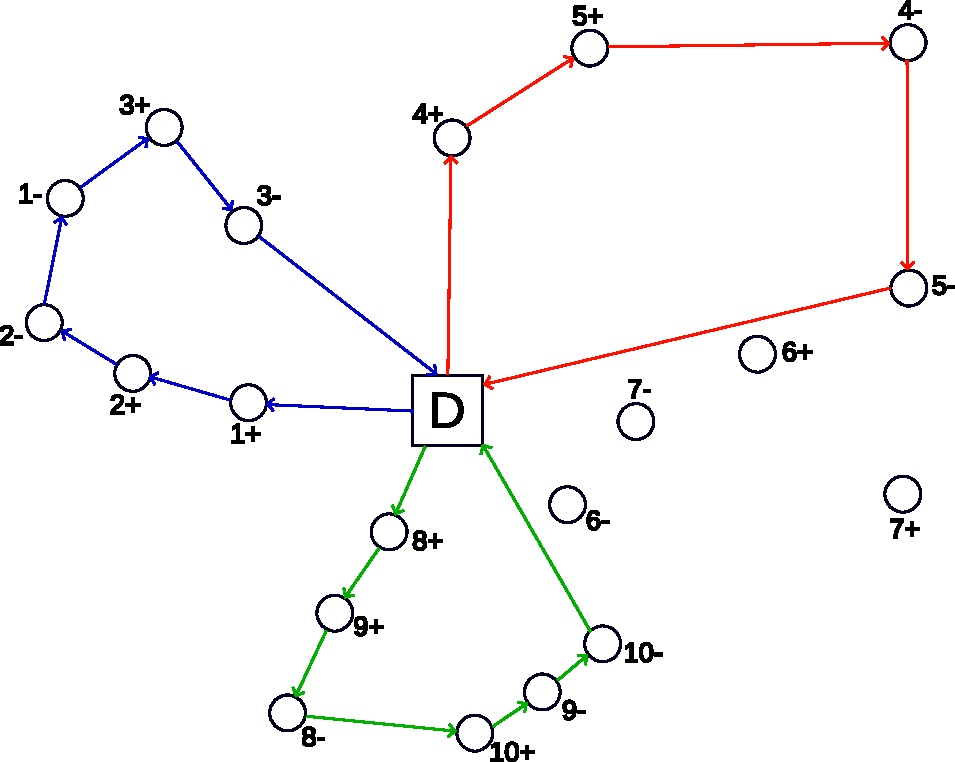
\includegraphics[width=\textwidth]{graphics/lns-destroy-solution} 
%	\captionof{figure}[]{Destroyed solution.}
%\end{figure}
%\end{minipage}%
%\hfill%
%\begin{minipage}[t]{.3\textwidth}
%\begin{figure}
%	\centering
%	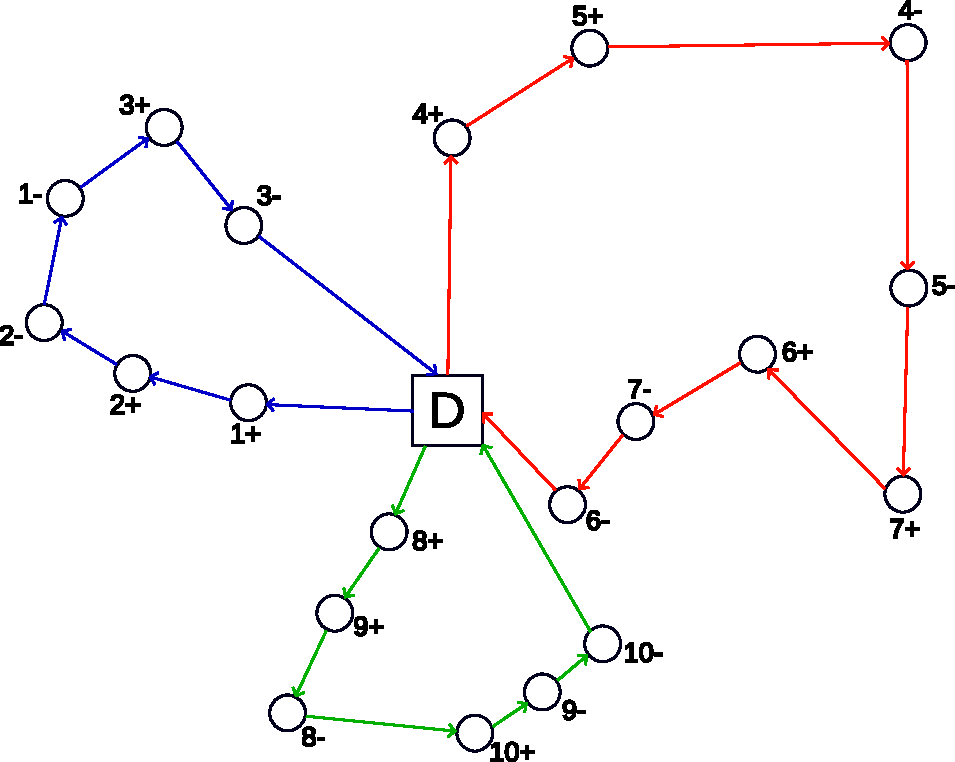
\includegraphics[width=\textwidth]{graphics/lns-repair-solution} 
%	\captionof{figure}[]{Repaired solution.}
%\end{figure}
%\end{minipage}%
% new figures without bold numbers 
\begin{minipage}[t]{0.3\linewidth}
\begin{figure}
	\centering
	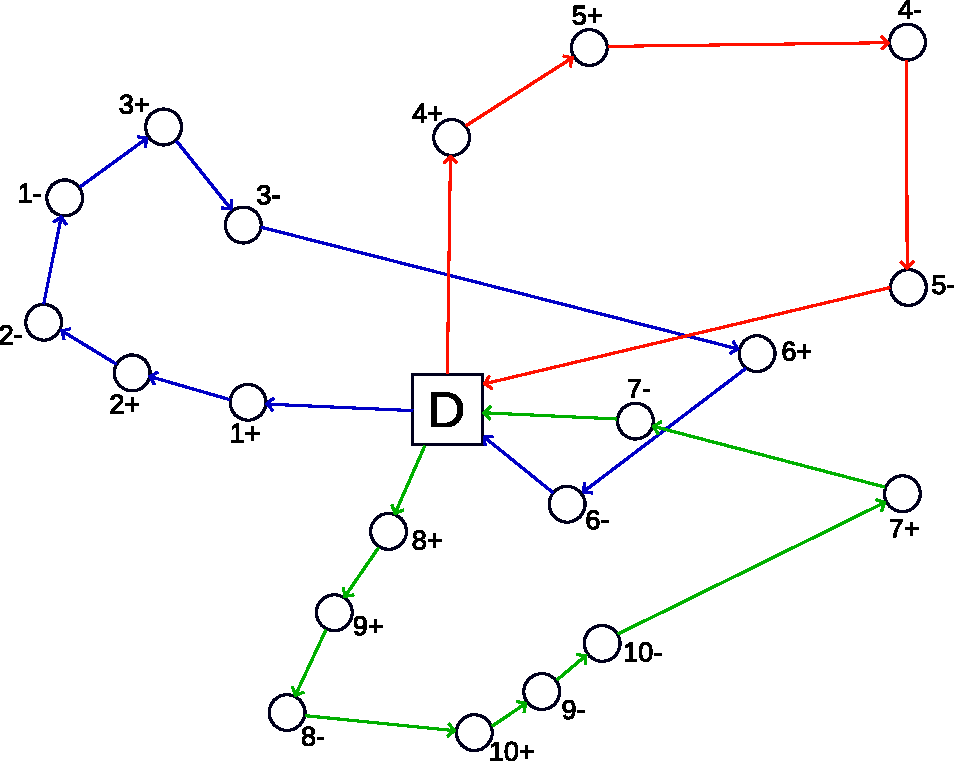
\includegraphics[width=\textwidth]{graphics/lns-initial-solution-new}
	\caption{Initial solution.}
\end{figure}
\end{minipage}%
\hfill%
\begin{minipage}[t]{.3\textwidth}
\begin{figure}
	\centering
	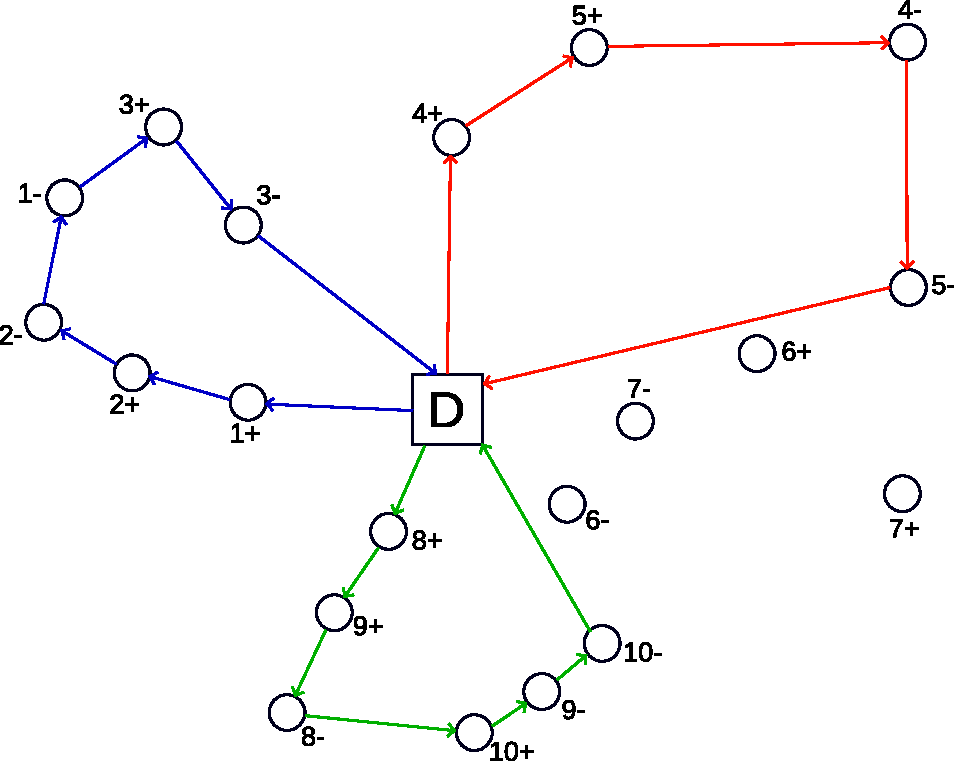
\includegraphics[width=\textwidth]{graphics/lns-destroy-solution-new} 
	\captionof{figure}[]{Destroyed solution.}
\end{figure}
\end{minipage}%
\hfill%
\begin{minipage}[t]{.3\textwidth}
\begin{figure}
	\centering
	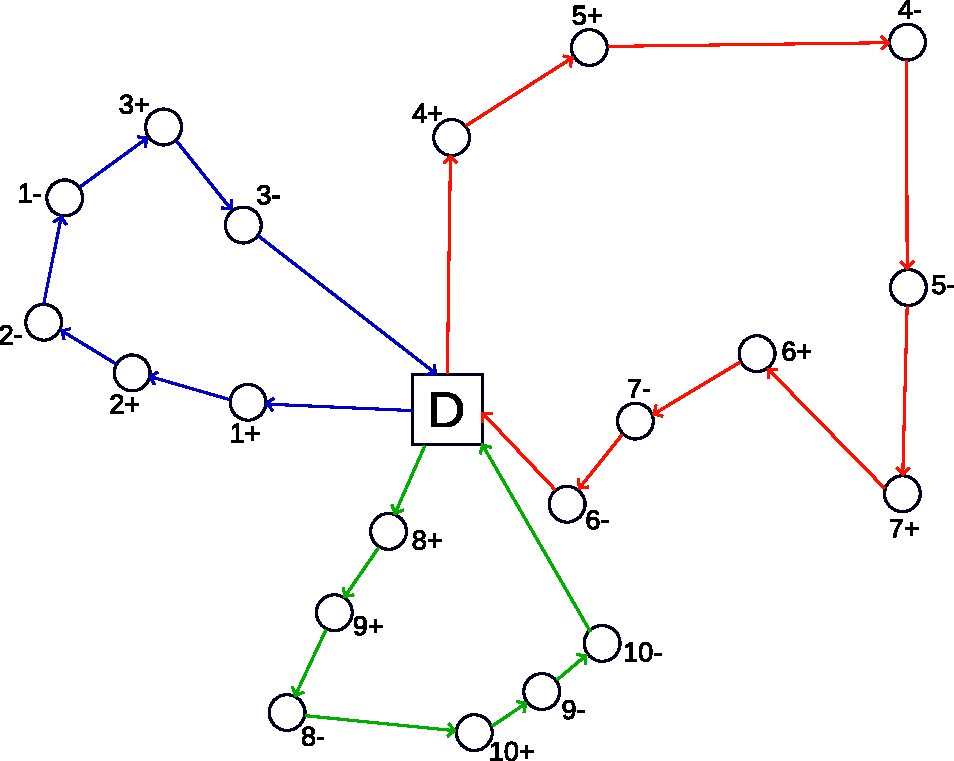
\includegraphics[width=\textwidth]{graphics/lns-repair-solution-new} 
	\captionof{figure}[]{Repaired solution.}
\end{figure}
\end{minipage}%

\bigskip

%\structure{Random removal} {\footnotesize{\textcolor{gray}{(\cite{Ropke:2006})}}}
%\begin{itemize}
%%	\item Remove 15 randomly selected requests 
%	\item Remove randomly selected requests 
%\end{itemize}

\structure{Destroy operator:} %random removal {\footnotesize{\textcolor{gray}{(\cite{Ropke:2006})}}}
\begin{itemize}
%	\item Remove 15 randomly selected requests 
	\item Remove uniformly randomly selected requests 
\end{itemize}


\end{frame}

\begin{frame}
  \frametitle{Large Neighborhood Search (LNS)}
  \framesubtitle{Repair Operators}
  
\structure{Greedy heuristic:}
\begin{itemize}
	\item Cheapest insertion over all unserved requests and routes 
\end{itemize}

\medskip

\structure{Time window order based heuristic:} %TODO or greedy heuristic based on time windows, similar to Limmer? 
\begin{itemize}
	\item Consider unserved requests in non-decreasing order of the start of the pickup time windows 
	\item Cheapest insertion over all routes 
\end{itemize}

\medskip

\structure{Random order based heuristic:} %TODO or greedy heuristic with random order
\begin{itemize}
	\item Consider unserved requests in random order
	\item Cheapest insertion over all routes 
\end{itemize}

%(done) mention cost noise? -> nope, no time 
%TODO insert figure of repair operator

\end{frame}


%(done) otf-approach for charging station insertion and evaluation: MILP, heuristic
\subsection{Evaluation and On-The-Fly Charging Stop Insertion}

\begin{frame}
	\frametitle{Large Neighborhood Search (LNS)}
	\framesubtitle{Route Evaluation With On-The-Fly Charging Stop Insertion}
	
%(done) fix spacing (more space)
\begin{itemize}
	\item \important{LNS does not (directly) deal with charging stops!}
	\medskip 
	\item Route evaluation procedure: 
		\smallskip
		\begin{itemize}
			\item Checks feasibility 
			\smallskip
			\item Inserts charging stops as needed on-the-fly
			\smallskip
%			\item Determines times (waiting, service, charging)
			\item Determines charging durations 
		\end{itemize}
\end{itemize}

%\medskip
\bigskip

%(done) maybe remove assumptions to save time 
%\structure{Assumptions:}
%\begin{itemize}
%	\item $\leq 1$ charging stops in between successive fragments or depots 
%	\item No time windows for charging stations 
%\end{itemize}
%
%\medskip

\structure{Allows} consideration of: 
\smallskip
\begin{itemize}
%	\item Limited number of usages of each charging station %(done) remove this first point to save time?
%	\item Individual charging speeds $\alpha_s$ at charging stations $s \in S$
	\item Individual charging speeds at charging stations
%		\begin{itemize}
%			\item[$\rightarrow$] not possible with labeling algorithm! 
%		\end{itemize}
\end{itemize}
	
\end{frame}


\begin{frame}
  \frametitle{MILP-Based Charging Stop Insertion}
  
\structure{Goals:}
\begin{itemize}
	\item Determine insertion positions and charging durations satisfying battery-related constraints 
	\item Minimize total detour length caused by new charging stops %newly inserted charging stations 
\end{itemize} 

\bigskip

\structure{Benefit:} 
\begin{itemize}
	\item Optimal: charging stations, insertion positions
%	\item Allows multiple charging stops per route  
\end{itemize}

\bigskip

\structure{Drawbacks:}
\begin{itemize}
	\item Computationally expensive, slow 
\end{itemize}

\end{frame}


%TODO maybe visualize workflow
\begin{frame}
  \frametitle{Heuristic Charging Stop Insertion}

\only<1>{
\structure{Workflow:}
\begin{itemize}
	\item Determine list of start depot, fragments, and end depot,\\
	check individual validity of each fragment
	\item \structure{Forward pass:} % determine  
		\begin{itemize}
			\item Earliest service start times~$t^\mathrm{early}$ and waiting durations~$d^\mathrm{wait}$
			\item Battery levels of vehicle 
			\item Latest stop $i^\mathrm{ch}$ before which charging is necessary 
		\end{itemize}
	\item \structure{Backward pass:} % determine 
		\begin{itemize}
			\item Latest service start times $t^\mathrm{late}$ and backward-waiting durations~$d^\mathrm{wait\_back}$
		\end{itemize}
\end{itemize}
}

\only<2>{
\structure{Workflow (continued):}
\begin{itemize}
	\item Charging not necessary: terminate $\rightarrow$ feasible route %set $t^\mathrm{early}$ as service times  
	\item Charging necessary: 
		\begin{itemize}
			\item Go backwards from $i^\mathrm{ch}$ 
			\item Check each possible position and charging station % for feasibility and charging amount 
		\end{itemize}
	\item No feasible insertion: terminate $\rightarrow$ infeasible route 
	\item Feasible insertions: select and insert stop 
		\begin{itemize}
			\item If available: feasible tour and minimum detour length
			\item Otherwise: most energy charged 
		\end{itemize}
	\item Update all affected service and waiting times and battery levels 
	\item Repeat 
\end{itemize}
}
  
\end{frame}


%TODO remove whole slide to save time? TBD
\begin{frame}
  \frametitle{Heuristic Charging Stop Insertion}
  \framesubtitle{Time-Efficient Heuristic II}
  
\begin{itemize}
%	\item Allows multiple charging stops per route
	\item Feasibility achievable with 1 charging stop possible:
	\smallskip
		\begin{itemize}
			\item Optimal insertion
			\smallskip
			\item Linear run time: $O(|R|)$
		\end{itemize}
	\bigskip
	\item Multiple charging stops necessary: 
	\smallskip
		\begin{itemize}
			\item Best insertion heuristic %{\footnotesize{\textcolor{gray}{(similar to \cite{Keskin:2016})}}}
			\smallskip
			\item Run time: $O(|R| \cdot n_{\mathrm{charging}})$ 
			\smallskip
			\item $n_{\mathrm{charging}}$ \dots number of inserted charging stations 
		\end{itemize}
\end{itemize}

% removed for time reasons
%\bigskip
%
%\structure{Option:} if improvement, apply MILP once at the end % for optimal insertion 
%\begin{itemize}
%	\item Only small further improvements 
%	\item Massive slowdown
%	\item[$\rightarrow$] \important{Discarded!}
%\end{itemize}

\end{frame}



% experiments and results: setup, benchmark instances, parameter tuning?, results
\section{Computational Study}

\subsection{Setup}
\begin{frame}
  \frametitle{Computational Study}
  \framesubtitle{Setup}
  
\begin{itemize}
	\item Implementation in $\mathtt{Julia\ 1.10.0}$
	\item $\mathtt{Gurobi\ 10.0.3}$ (single-threaded) via $\mathtt{JuMP}$
	\item Runs per instance: 30 
	\item Time limit: 300\,s
	\item Memory limit: 20\,GB
	\item Intel Xeon E5-2640 v4 with 2.4\,GHz
\end{itemize}

\end{frame}

%(done) slide for parameter tuning? -> probably not
% noise is not mentioned, destroy rates for charging stations not mentioned (because separation-based approach not described), and only for request destroy rate not necessary I think -> mention at destroy operator

\begin{frame}
  \frametitle{Computational Study}
  \framesubtitle{Benchmark Instances}
  
\renewcommand*{\thefootnote}{\alph{footnote}} % footnote symbol: lower case alphabet
%\setbeamerfont{footnote}{size=\oldfootnotesize}
%\setbeamerfont{footnote}{size=\normalsize} % slightly larger than \oldfootnotesize
%\setbeamerfont{footnote}{size=\small} % footnotesize bit larger than \oldfootnotesize?
%\renewcommand*{\footnotesize}{\oldfootnotesize\fontsize{2.5}{4}\selectfont}
%\setbeamerfont{footnote}{size=\fontsize{7.5}{4}}
\setbeamerfont{footnote}{size=\oldfootnotesize}
\begin{itemize}
	\item 2 data sets:
		\begin{itemize}
%			\item 14 Cordeau instances~\cite{Cordeau:2006}: 2--5 vehicles, 16--50 requests 
%			\item 10 Ropke instances~\cite{Ropke:2007}: 5--8 vehicles, 48--96 requests 
%			\item[$\rightarrow$] enhanced with E-ADARP features~\cite{Bongiovanni:2019}
			\item 14 Cordeau instances\footnote[frame]{DARP instances by \cite{Cordeau:2006}}: 2--5 vehicles, 16--50 requests 
			\item 10 Ropke instances\footnote[frame]{DARP instances by \cite{Ropke:2007}}: 5--8 vehicles, 48--96 requests 
			\item[$\rightarrow$] enhanced with E-ADARP features\footnote[frame]{cf. \cite{Bongiovanni:2019}}
		\end{itemize}
	\bigskip
	\item 2 modes for charging station visits: 
		\begin{itemize}
			\item 1 visit per station: $n_\mathrm{s} = 1$
			\item Unlimited visits per station: $n_\mathrm{s} = \infty$
		\end{itemize}
	\bigskip
	\item 3 minimum battery level ratios: $\gamma \in \{0.1, 0.4, 0.7\}$
\end{itemize}

\end{frame}


% alternative slide with list of literature approaches to avoid the references in the tables?
% -> nope, too much on one slide. Try separate slide instead!
% or simple remove references? but e-ADARP2 is not mentioned anywhere else...
% => result: add e-ADARP2 to related work, remove literature approaches here and remove citations in table

\subsection{Results}


% alternative2: removed columns with standard deviation and columns with number of feasible solutions
% new version without citations 
\begin{frame}
  \frametitle{Results: Cordeau instances with $\gamma = 0.1$}
  
%\setlength{\intextsep}{0.1\baselineskip}
  
%NEW2: Cordeau instances with $\gamma = 0.1$


% Please add the following required packages to your document preamble:
% \usepackage{multirow}
% \usepackage{graphicx}
% \usepackage[table,xcdraw]{xcolor}
% Beamer presentation requires \usepackage{colortbl} instead of \usepackage[table,xcdraw]{xcolor}
\begin{table}[]
\centering
\normalsize
%\caption{Results on Cordeau instances with $\gamma = 0.1$ for limited CS visits ($n_\mathrm{s} = 1$) and unlimited CS visits ($n_\mathrm{s} = \infty$).  }
%\caption{ Cordeau instances with $\gamma = 0.1$}
\label{tab:eurocast24_results_cordeau_g01}
\resizebox{0.9\columnwidth}{!}{%
\begin{tabular}{lrrrrrrrrrrr}
\hline
\multicolumn{1}{c}{}                           & \multicolumn{2}{c}{\begin{tabular}[c]{@{}c@{}}e-ADARP2\end{tabular}} & \multicolumn{3}{c}{\begin{tabular}[c]{@{}c@{}}DA\end{tabular}}                                                                 & \multicolumn{2}{c}{\begin{tabular}[c]{@{}c@{}}BI-LNS\end{tabular}} & \multicolumn{2}{c}{\begin{tabular}[c]{@{}c@{}}OTF MILP\end{tabular}} & \multicolumn{2}{c}{\begin{tabular}[c]{@{}c@{}}OTF Heuristic\end{tabular}} \\ \cline{2-12} %\cmidrule{2-12}%
\multicolumn{1}{c}{\multirow{-2}{*}{Instance}} & \begin{tabular}[c]{@{}r@{}}RT {[}min{]}\end{tabular} & \multicolumn{1}{r|}{Obj}             & \begin{tabular}[c]{@{}r@{}}RT mean {[}min{]}\end{tabular} & Obj min         & \multicolumn{1}{r|}{Obj mean}                               & Obj min             & \multicolumn{1}{r|}{Obj mean}                                  & Obj min           & \multicolumn{1}{r|}{Obj mean}                                & Obj min                       & Obj mean                                             \\ \hline
\multicolumn{12}{c}{$n_\mathrm{s} = 1$}                                                                                                                                                                                                                                                                                                                                                                                                                                                                                                                         \\ \hline
a2-16                                          & 0.02                                                    & \multicolumn{1}{r|}{\textbf{237.38}} & 0.65                                                         & \textbf{237.38} & \multicolumn{1}{r|}{{\color[HTML]{FE0000} \textbf{237.38}}} & 238.20              & \multicolumn{1}{r|}{238.20}                                    & \textbf{237.38}   & \multicolumn{1}{r|}{{\color[HTML]{FE0000} \textbf{237.38}}}  & \textbf{237.38}               & {\color[HTML]{FE0000} \textbf{237.38}}               \\
a2-20                                          & 0.07                                                    & \multicolumn{1}{r|}{\textbf{279.08}} & 1.23                                                         & \textbf{279.08} & \multicolumn{1}{r|}{{\color[HTML]{FE0000} \textbf{279.08}}} & 281.00              & \multicolumn{1}{r|}{281.00}                                    & \textbf{279.08}   & \multicolumn{1}{r|}{{\color[HTML]{FE0000} \textbf{279.08}}}  & \textbf{279.08}               & {\color[HTML]{FE0000} \textbf{279.08}}               \\
a2-24                                          & 0.15                                                    & \multicolumn{1}{r|}{\textbf{346.21}} & 2.68                                                         & \textbf{346.21} & \multicolumn{1}{r|}{{\color[HTML]{FE0000} \textbf{346.21}}} & \textbf{346.21}     & \multicolumn{1}{r|}{346.59}                                    & \textbf{346.21}   & \multicolumn{1}{r|}{346.66}                                  & \textbf{346.21}               & {\color[HTML]{FE0000} \textbf{346.21}}               \\
a3-18                                          & 0.08                                                    & \multicolumn{1}{r|}{236.82}          & 0.42                                                         & 236.82          & \multicolumn{1}{r|}{236.82}                                 & 238.73              & \multicolumn{1}{r|}{238.75}                                    & \textbf{236.81}   & \multicolumn{1}{r|}{{\color[HTML]{FE0000} \textbf{236.81}}}  & \textbf{236.81}               & {\color[HTML]{FE0000} \textbf{236.81}}               \\
a3-24                                          & 0.23                                                    & \multicolumn{1}{r|}{\textbf{274.80}} & 0.97                                                         & \textbf{274.80} & \multicolumn{1}{r|}{{\color[HTML]{FE0000} \textbf{274.80}}} & 275.18              & \multicolumn{1}{r|}{275.18}                                    & \textbf{274.80}   & \multicolumn{1}{r|}{275.50}                                  & \textbf{274.80}               & {\color[HTML]{FE0000} \textbf{274.80}}               \\
a3-30                                          & 1.70                                                    & \multicolumn{1}{r|}{\textbf{413.27}} & 0.90                                                         & \textbf{413.27} & \multicolumn{1}{r|}{{\color[HTML]{FE0000} \textbf{413.27}}} & 414.88              & \multicolumn{1}{r|}{414.88}                                    & \textbf{413.27}   & \multicolumn{1}{r|}{414.33}                                  & \textbf{413.27}               & {\color[HTML]{FE0000} \textbf{413.27}}               \\
a3-36                                          & 1.78                                                    & \multicolumn{1}{r|}{\textbf{481.17}} & 2.54                                                         & \textbf{481.17} & \multicolumn{1}{r|}{{\color[HTML]{FE0000} \textbf{481.17}}} & 483.86              & \multicolumn{1}{r|}{484.05}                                    & 481.38            & \multicolumn{1}{r|}{486.09}                                  & \textbf{481.17}               & 482.18                                               \\
a4-16                                          & 0.06                                                    & \multicolumn{1}{r|}{\textbf{222.49}} & 0.32                                                         & \textbf{222.49} & \multicolumn{1}{r|}{{\color[HTML]{FE0000} \textbf{222.49}}} & \textbf{222.49}     & \multicolumn{1}{r|}{{\color[HTML]{FE0000} \textbf{222.49}}}    & \textbf{222.49}   & \multicolumn{1}{r|}{222.61}                                  & \textbf{222.49}               & {\color[HTML]{FE0000} \textbf{222.49}}               \\
a4-24                                          & 0.52                                                    & \multicolumn{1}{r|}{\textbf{310.84}} & 0.49                                                         & \textbf{310.84} & \multicolumn{1}{r|}{{\color[HTML]{FE0000} \textbf{310.84}}} & 311.48              & \multicolumn{1}{r|}{311.48}                                    & \textbf{310.84}   & \multicolumn{1}{r|}{310.95}                                  & \textbf{310.84}               & {\color[HTML]{FE0000} \textbf{310.84}}               \\
a4-32                                          & 10.20                                                   & \multicolumn{1}{r|}{393.96}          & 0.87                                                         & 393.96          & \multicolumn{1}{r|}{395.12}                                 & 394.66              & \multicolumn{1}{r|}{394.79}                                    & \textbf{393.95}   & \multicolumn{1}{r|}{394.89}                                  & \textbf{393.95}               & {\color[HTML]{FE0000} \textbf{393.95}}               \\
a4-40                                          & 8.62                                                    & \multicolumn{1}{r|}{\textbf{453.84}} & 1.53                                                         & \textbf{453.84} & \multicolumn{1}{r|}{459.42}                                 & 456.93              & \multicolumn{1}{r|}{457.08}                                    & \textbf{453.84}   & \multicolumn{1}{r|}{462.55}                                  & \textbf{453.84}               & {\color[HTML]{FE0000} \textbf{454.46}}               \\
a4-48                                          & 120.00                                                  & \multicolumn{1}{r|}{\textbf{554.54}} & 2.36                                                         & 555.93          & \multicolumn{1}{r|}{561.26}                                 & 557.24              & \multicolumn{1}{r|}{557.94}                                    & 556.36            & \multicolumn{1}{r|}{560.02}                                  & \textbf{554.54}               & {\color[HTML]{FE0000} \textbf{555.38}}               \\
a5-40                                          & 19.03                                                   & \multicolumn{1}{r|}{414.51}          & 1.08                                                         & 414.80          & \multicolumn{1}{r|}{420.35}                                 & 415.62              & \multicolumn{1}{r|}{415.65}                                    & 415.80            & \multicolumn{1}{r|}{422.04}                                  & \textbf{414.50}               & {\color[HTML]{FE0000} \textbf{414.99}}               \\
a5-50                                          & 120.00                                                  & \multicolumn{1}{r|}{\textbf{559.17}} & 2.29                                                         & 561.41          & \multicolumn{1}{r|}{570.58}                                 & 560.07              & \multicolumn{1}{r|}{{\color[HTML]{FE0000} \textbf{560.66}}}    & 563.50            & \multicolumn{1}{r|}{571.47}                                  & \textbf{559.17}               & 562.18                                               \\ \hline
\multicolumn{12}{c}{$n_\mathrm{s} = \infty$}                                                                                                                                                                                                                                                                                                                                                                                                                                                                                                                    \\ \hline
a2-16                                          &                                                         & \multicolumn{1}{r|}{}                &                                                              & \textbf{}       & \multicolumn{1}{r|}{}                                       & 238.20              & \multicolumn{1}{r|}{238.20}                                    & \textbf{237.38}   & \multicolumn{1}{r|}{{\color[HTML]{FE0000} \textbf{237.38}}}  & \textbf{237.38}               & {\color[HTML]{FE0000} \textbf{237.38}}               \\
a2-20                                          &                                                         & \multicolumn{1}{r|}{}                &                                                              &                 & \multicolumn{1}{r|}{}                                       & 281.00              & \multicolumn{1}{r|}{281.00}                                    & \textbf{279.08}   & \multicolumn{1}{r|}{{\color[HTML]{FE0000} \textbf{279.08}}}  & \textbf{279.08}               & {\color[HTML]{FE0000} \textbf{279.08}}               \\
a2-24                                          &                                                         & \multicolumn{1}{r|}{}                &                                                              &                 & \multicolumn{1}{r|}{}                                       & \textbf{346.21}     & \multicolumn{1}{r|}{346.22}                                    & \textbf{346.21}   & \multicolumn{1}{r|}{346.39}                                  & \textbf{346.21}               & {\color[HTML]{FE0000} \textbf{346.21}}               \\
a3-18                                          &                                                         & \multicolumn{1}{r|}{}                &                                                              & \textbf{}       & \multicolumn{1}{r|}{}                                       & 238.73              & \multicolumn{1}{r|}{238.73}                                    & \textbf{236.81}   & \multicolumn{1}{r|}{{\color[HTML]{FE0000} \textbf{236.81}}}  & \textbf{236.81}               & {\color[HTML]{FE0000} \textbf{236.81}}               \\
a3-24                                          &                                                         & \multicolumn{1}{r|}{}                &                                                              & \textbf{}       & \multicolumn{1}{r|}{}                                       & 275.18              & \multicolumn{1}{r|}{275.18}                                    & \textbf{274.80}   & \multicolumn{1}{r|}{275.60}                                  & \textbf{274.80}               & {\color[HTML]{FE0000} \textbf{274.80}}               \\
a3-30                                          &                                                         & \multicolumn{1}{r|}{}                &                                                              &                 & \multicolumn{1}{r|}{}                                       & 414.88              & \multicolumn{1}{r|}{414.88}                                    & \textbf{413.27}   & \multicolumn{1}{r|}{414.92}                                  & \textbf{413.27}               & {\color[HTML]{FE0000} \textbf{413.27}}               \\
a3-36                                          &                                                         & \multicolumn{1}{r|}{}                &                                                              &                 & \multicolumn{1}{r|}{}                                       & 483.86              & \multicolumn{1}{r|}{483.86}                                    & \textbf{481.17}   & \multicolumn{1}{r|}{486.63}                                  & \textbf{481.17}               & {\color[HTML]{FE0000} \textbf{482.26}}               \\
a4-16                                          &                                                         & \multicolumn{1}{r|}{}                &                                                              & \textbf{}       & \multicolumn{1}{r|}{}                                       & \textbf{222.49}     & \multicolumn{1}{r|}{{\color[HTML]{FE0000} \textbf{222.49}}}    & \textbf{222.49}   & \multicolumn{1}{r|}{222.78}                                  & \textbf{222.49}               & {\color[HTML]{FE0000} \textbf{222.49}}               \\
a4-24                                          &                                                         & \multicolumn{1}{r|}{}                &                                                              &                 & \multicolumn{1}{r|}{}                                       & 311.48              & \multicolumn{1}{r|}{311.48}                                    & \textbf{310.84}   & \multicolumn{1}{r|}{310.96}                                  & \textbf{310.84}               & {\color[HTML]{FE0000} \textbf{310.84}}               \\
a4-32                                          &                                                         & \multicolumn{1}{r|}{}                &                                                              & \textbf{}       & \multicolumn{1}{r|}{}                                       & 394.66              & \multicolumn{1}{r|}{394.79}                                    & \textbf{393.95}   & \multicolumn{1}{r|}{394.64}                                  & \textbf{393.95}               & {\color[HTML]{FE0000} \textbf{393.95}}               \\
a4-40                                          &                                                         & \multicolumn{1}{r|}{}                &                                                              &                 & \multicolumn{1}{r|}{}                                       & 456.93              & \multicolumn{1}{r|}{457.37}                                    & 455.26            & \multicolumn{1}{r|}{462.06}                                  & \textbf{453.84}               & {\color[HTML]{FE0000} \textbf{453.84}}               \\
a4-48                                          &                                                         & \multicolumn{1}{r|}{}                &                                                              &                 & \multicolumn{1}{r|}{}                                       & 557.25              & \multicolumn{1}{r|}{557.82}                                    & 555.70            & \multicolumn{1}{r|}{560.01}                                  & \textbf{554.54}               & {\color[HTML]{FE0000} \textbf{555.43}}               \\
a5-40                                          &                                                         & \multicolumn{1}{r|}{}                &                                                              &                 & \multicolumn{1}{r|}{}                                       & 415.62              & \multicolumn{1}{r|}{415.62}                                    & 416.45            & \multicolumn{1}{r|}{422.27}                                  & \textbf{414.50}               & {\color[HTML]{FE0000} \textbf{415.13}}               \\
a5-50                                          &                                                         & \multicolumn{1}{r|}{}                &                                                              &                 & \multicolumn{1}{r|}{}                                       & 560.07              & \multicolumn{1}{r|}{{\color[HTML]{FE0000} \textbf{560.95}}}    & 563.87            & \multicolumn{1}{r|}{571.30}                                  & \textbf{559.17}               & 561.81                                               \\ \hline
\end{tabular}%
}
\end{table}

\end{frame}

% alternative2: removed columns with standard deviation and columns with number of feasible solutions
% new version: without citations 
\begin{frame}
  \frametitle{Results: Cordeau instances with $\gamma = 0.7$ }
  

% Please add the following required packages to your document preamble:
% \usepackage{multirow}
% \usepackage{graphicx}
% \usepackage[table,xcdraw]{xcolor}
% Beamer presentation requires \usepackage{colortbl} instead of \usepackage[table,xcdraw]{xcolor}
\begin{table}[]
\centering
%\caption{Results on Cordeau instances with $\gamma = 0.7$ for limited CS visits ($n_\mathrm{s} = 1$) and unlimited CS visits ($n_\mathrm{s} = \infty$).  }
\label{tab:eurocast24_results_cordeau_g07}
\resizebox{0.9\textwidth}{!}{%
\begin{tabular}{lrrrrrrrrrrr}
\hline
\multicolumn{1}{c}{}                           & \multicolumn{2}{c}{e-ADARP2}                                 & \multicolumn{3}{c}{DA}                                                                       & \multicolumn{2}{c}{BI-LNS}             & \multicolumn{2}{c}{OTF MILP}                                                  & \multicolumn{2}{c}{OTF Heuristic}                        \\ \cline{2-12} 
\multicolumn{1}{c}{\multirow{-2}{*}{Instance}} & RT {[}min{]} & \multicolumn{1}{r|}{Obj}                                    & RT mean {[}min{]} & Obj min         & \multicolumn{1}{r|}{Obj mean}                               & Obj min         & \multicolumn{1}{r|}{Obj mean} & Obj min         & \multicolumn{1}{r|}{Obj mean}                               & Obj min         & Obj mean                               \\ \hline
\multicolumn{12}{c}{$n_\mathrm{s} = 1$}                                                                                                                                                                                                                                                                                                                                                                                      \\ \hline
a2-16                                          & 0.09         & \multicolumn{1}{r|}{{\color[HTML]{000000} \textbf{240.66}}} & 1.60              & \textbf{240.66} & \multicolumn{1}{r|}{{\color[HTML]{FE0000} \textbf{240.66}}} & 242.83          & \multicolumn{1}{r|}{245.50}   & \textbf{240.66} & \multicolumn{1}{r|}{240.84}                                 & \textbf{240.66} & {\color[HTML]{FE0000} \textbf{240.66}} \\
a2-20                                          & 120.00       & \multicolumn{1}{r|}{NA}                                     & 2.88              & \textbf{293.27} & \multicolumn{1}{r|}{294.11}                                 & NA              & \multicolumn{1}{r|}{NA}       & \textbf{293.27} & \multicolumn{1}{r|}{294.98}                                 & \textbf{293.27} & {\color[HTML]{FE0000} \textbf{293.27}} \\
a2-24                                          & 16.02        & \multicolumn{1}{r|}{358.21}                                 & 3.44              & \textbf{353.18} & \multicolumn{1}{r|}{NA}                                     & 356.99          & \multicolumn{1}{r|}{363.04}   & \textbf{353.18} & \multicolumn{1}{r|}{353.45}                                 & \textbf{353.18} & {\color[HTML]{FE0000} \textbf{353.18}} \\
a3-18                                          & 0.80         & \multicolumn{1}{r|}{\textbf{240.58}}                        & 0.97              & \textbf{240.58} & \multicolumn{1}{r|}{{\color[HTML]{FE0000} \textbf{240.58}}} & 242.49          & \multicolumn{1}{r|}{246.13}   & \textbf{240.58} & \multicolumn{1}{r|}{240.98}                                 & \textbf{240.58} & {\color[HTML]{FE0000} \textbf{240.58}} \\
a3-24                                          & 2.54         & \multicolumn{1}{r|}{277.72}                                 & 2.06              & \textbf{275.97} & \multicolumn{1}{r|}{277.43}                                 & 277.52          & \multicolumn{1}{r|}{277.52}   & \textbf{275.97} & \multicolumn{1}{r|}{277.46}                                 & \textbf{275.97} & {\color[HTML]{FE0000} \textbf{275.97}} \\
a3-30                                          & 120.00       & \multicolumn{1}{r|}{NA}                                     & 1.30              & \textbf{424.93} & \multicolumn{1}{r|}{436.20}                                 & 432.27          & \multicolumn{1}{r|}{436.56}   & \textbf{424.93} & \multicolumn{1}{r|}{430.32}                                 & \textbf{424.93} & {\color[HTML]{FE0000} \textbf{426.12}} \\
a3-36                                          & 120.00       & \multicolumn{1}{r|}{\textbf{494.04}}                        & 2.09              & \textbf{494.04} & \multicolumn{1}{r|}{502.27}                                 & 496.75          & \multicolumn{1}{r|}{500.84}   & \textbf{494.04} & \multicolumn{1}{r|}{502.35}                                 & \textbf{494.04} & {\color[HTML]{FE0000} \textbf{497.18}} \\
a4-16                                          & 1.12         & \multicolumn{1}{r|}{\textbf{223.13}}                        & 0.52              & \textbf{223.13} & \multicolumn{1}{r|}{{\color[HTML]{FE0000} \textbf{223.13}}} & \textbf{223.13} & \multicolumn{1}{r|}{223.95}   & \textbf{223.13} & \multicolumn{1}{r|}{223.37}                                 & \textbf{223.13} & {\color[HTML]{FE0000} \textbf{223.13}} \\
a4-24                                          & 30.58        & \multicolumn{1}{r|}{318.21}                                 & 0.90              & \textbf{316.65} & \multicolumn{1}{r|}{318.31}                                 & 319.37          & \multicolumn{1}{r|}{321.10}   & \textbf{316.65} & \multicolumn{1}{r|}{319.17}                                 & \textbf{316.65} & {\color[HTML]{FE0000} \textbf{316.65}} \\
a4-32                                          & 120.00       & \multicolumn{1}{r|}{430.07}                                 & 1.19              & \textbf{397.87} & \multicolumn{1}{r|}{405.85}                                 & 401.97          & \multicolumn{1}{r|}{402.59}   & \textbf{397.87} & \multicolumn{1}{r|}{399.98}                                 & \textbf{397.87} & {\color[HTML]{FE0000} \textbf{397.87}} \\
a4-40                                          & 120.00       & \multicolumn{1}{r|}{NA}                                     & 1.91              & 479.02          & \multicolumn{1}{r|}{NA}                                     & 471.72          & \multicolumn{1}{r|}{478.93}   & 471.78          & \multicolumn{1}{r|}{487.42}                                 & \textbf{467.72} & {\color[HTML]{FE0000} \textbf{474.47}} \\
a4-48                                          & 120.00       & \multicolumn{1}{r|}{NA}                                     & 2.74              & 582.22          & \multicolumn{1}{r|}{NA}                                     & 579.71          & \multicolumn{1}{r|}{588.48}   & 580.49          & \multicolumn{1}{r|}{591.36}                                 & \textbf{575.62} & {\color[HTML]{FE0000} \textbf{579.63}} \\
a5-40                                          & 120.00       & \multicolumn{1}{r|}{447.63}                                 & 1.63              & 424.26          & \multicolumn{1}{r|}{436.94}                                 & 420.20          & \multicolumn{1}{r|}{423.88}   & 425.93          & \multicolumn{1}{r|}{433.02}                                 & \textbf{418.75} & {\color[HTML]{FE0000} \textbf{421.16}} \\
a5-50                                          & 120.00       & \multicolumn{1}{r|}{NA}                                     & 2.64              & 603.24          & \multicolumn{1}{r|}{NA}                                     & 593.71          & \multicolumn{1}{r|}{602.30}   & 596.54          & \multicolumn{1}{r|}{612.00}                                 & \textbf{589.61} & {\color[HTML]{FE0000} \textbf{596.09}} \\ \hline
\multicolumn{12}{c}{$n_\mathrm{s} = \infty$}                                                                                                                                                                                                                                                                                                                                                                                 \\ \hline
a2-16                                          &              & \multicolumn{1}{r|}{}                                       & 1.99              & \textbf{240.66} & \multicolumn{1}{r|}{{\color[HTML]{FE0000} \textbf{240.66}}} & 242.44          & \multicolumn{1}{r|}{242.44}   & \textbf{240.66} & \multicolumn{1}{r|}{{\color[HTML]{FE0000} \textbf{240.66}}} & \textbf{240.66} & {\color[HTML]{FE0000} \textbf{240.66}} \\
a2-20                                          &              & \multicolumn{1}{r|}{}                                       & 5.27              & 286.32          & \multicolumn{1}{r|}{288.89}                                 & 290.33          & \multicolumn{1}{r|}{291.23}   & \textbf{285.86} & \multicolumn{1}{r|}{285.95}                                 & \textbf{285.86} & {\color[HTML]{FE0000} \textbf{285.86}} \\
a2-24                                          &              & \multicolumn{1}{r|}{}                                       & 5.96              & 354.38          & \multicolumn{1}{r|}{374.68}                                 & 354.53          & \multicolumn{1}{r|}{356.89}   & \textbf{350.32} & \multicolumn{1}{r|}{350.33}                                 & \textbf{350.32} & {\color[HTML]{FE0000} \textbf{350.32}} \\
a3-18                                          &              & \multicolumn{1}{r|}{}                                       & 1.10              & \textbf{238.82} & \multicolumn{1}{r|}{{\color[HTML]{FE0000} \textbf{238.82}}} & 241.95          & \multicolumn{1}{r|}{242.46}   & \textbf{238.82} & \multicolumn{1}{r|}{239.55}                                 & 240.03          & 240.03                                 \\
a3-24                                          &              & \multicolumn{1}{r|}{}                                       & 2.50              & \textbf{275.20} & \multicolumn{1}{r|}{{\color[HTML]{FE0000} \textbf{275.20}}} & 277.52          & \multicolumn{1}{r|}{278.02}   & \textbf{275.20} & \multicolumn{1}{r|}{276.05}                                 & \textbf{275.20} & {\color[HTML]{FE0000} \textbf{275.20}} \\
a3-30                                          &              & \multicolumn{1}{r|}{}                                       & 2.85              & 415.71          & \multicolumn{1}{r|}{417.07}                                 & 419.16          & \multicolumn{1}{r|}{426.30}   & \textbf{413.45} & \multicolumn{1}{r|}{415.85}                                 & \textbf{413.45} & {\color[HTML]{FE0000} \textbf{414.08}} \\
a3-36                                          &              & \multicolumn{1}{r|}{}                                       & 5.72              & 484.85          & \multicolumn{1}{r|}{487.91}                                 & 490.26          & \multicolumn{1}{r|}{492.79}   & \textbf{483.08} & \multicolumn{1}{r|}{490.60}                                 & 484.49          & {\color[HTML]{FE0000} \textbf{486.98}} \\
a4-16                                          &              & \multicolumn{1}{r|}{}                                       & 0.52              & \textbf{222.49} & \multicolumn{1}{r|}{{\color[HTML]{FE0000} \textbf{222.49}}} & \textbf{222.49} & \multicolumn{1}{r|}{223.57}   & \textbf{222.49} & \multicolumn{1}{r|}{223.09}                                 & \textbf{222.49} & {\color[HTML]{FE0000} \textbf{222.49}} \\
a4-24                                          &              & \multicolumn{1}{r|}{}                                       & 1.18              & 315.98          & \multicolumn{1}{r|}{317.99}                                 & 316.51          & \multicolumn{1}{r|}{318.38}   & \textbf{315.40} & \multicolumn{1}{r|}{316.00}                                 & 315.98          & {\color[HTML]{FE0000} \textbf{315.98}} \\
a4-32                                          &              & \multicolumn{1}{r|}{}                                       & 2.06              & \textbf{394.94} & \multicolumn{1}{r|}{401.82}                                 & 396.64          & \multicolumn{1}{r|}{397.98}   & \textbf{394.94} & \multicolumn{1}{r|}{395.84}                                 & \textbf{394.94} & {\color[HTML]{FE0000} \textbf{394.94}} \\
a4-40                                          &              & \multicolumn{1}{r|}{}                                       & 3.77              & 458.52          & \multicolumn{1}{r|}{467.60}                                 & 461.16          & \multicolumn{1}{r|}{461.91}   & \textbf{457.76} & \multicolumn{1}{r|}{465.13}                                 & 457.88          & {\color[HTML]{FE0000} \textbf{458.67}} \\
a4-48                                          &              & \multicolumn{1}{r|}{}                                       & 6.72              & 568.08          & \multicolumn{1}{r|}{575.96}                                 & 568.01          & \multicolumn{1}{r|}{570.80}   & \textbf{561.15} & \multicolumn{1}{r|}{565.94}                                 & 561.38          & {\color[HTML]{FE0000} \textbf{564.54}} \\
a5-40                                          &              & \multicolumn{1}{r|}{}                                       & 2.50              & 419.33          & \multicolumn{1}{r|}{425.29}                                 & 418.79          & \multicolumn{1}{r|}{421.06}   & \textbf{415.88} & \multicolumn{1}{r|}{425.07}                                 & \textbf{415.88} & {\color[HTML]{FE0000} \textbf{416.43}} \\
a5-50                                          &              & \multicolumn{1}{r|}{}                                       & 5.88              & 579.15          & \multicolumn{1}{r|}{588.98}                                 & 571.37          & \multicolumn{1}{r|}{575.49}   & 573.37          & \multicolumn{1}{r|}{586.47}                                 & \textbf{567.61} & {\color[HTML]{FE0000} \textbf{571.48}} \\ \hline
\end{tabular}%
}
\end{table}

\end{frame}


% alternative: removed columns with standard deviation 
% new version: without citations 
\begin{frame}
  \frametitle{Results: Ropke instances with $\gamma = 0.1$}
  

% Please add the following required packages to your document preamble:
% \usepackage{multirow}
% \usepackage{graphicx}
% \usepackage[table,xcdraw]{xcolor}
% Beamer presentation requires \usepackage{colortbl} instead of \usepackage[table,xcdraw]{xcolor}
\begin{table}[]
\centering
%\caption{Results on Ropke instances with $\gamma = 0.1$ for limited CS visits ($n_\mathrm{s} = 1$) and unlimited CS visits ($n_\mathrm{s} = \infty$).  }
\label{tab:eurocast24_results_ropke_g01}
\resizebox{0.92\textwidth}{!}{%
\begin{tabular}{lrrrrrrrrr}
\hline
\multicolumn{1}{c}{}                           & \multicolumn{3}{c}{DA}                                 & \multicolumn{3}{c}{OTF MILP}                    & \multicolumn{3}{c}{OTF Heuristic}                                  \\ \cline{2-10} 
\multicolumn{1}{c}{\multirow{-2}{*}{Instance}} & RT mean {[}min{]} & Obj min & \multicolumn{1}{r|}{Obj mean} & Obj min & Obj mean & \multicolumn{1}{r|}{Feas}  & Obj min          & Obj mean                                & Feas  \\ \hline
\multicolumn{10}{c}{$n_\mathrm{s} = 1$}                                                                                                                                                                                             \\ \hline
a5-60                                          & 2.97              & 691.83  & \multicolumn{1}{r|}{706.20}   & 689.73  & 697.36   & \multicolumn{1}{r|}{30/30} & \textbf{683.87}  & {\color[HTML]{FE0000} \textbf{687.42}}  & 30/30 \\
a6-48                                          & 3.82              & 506.72  & \multicolumn{1}{r|}{512.69}   & 507.51  & 515.37   & \multicolumn{1}{r|}{30/30} & \textbf{506.45}  & {\color[HTML]{FE0000} \textbf{506.77}}  & 30/30 \\
a6-60                                          & 2.12              & 692.00  & \multicolumn{1}{r|}{700.15}   & 695.27  & 705.03   & \multicolumn{1}{r|}{30/30} & \textbf{690.29}  & {\color[HTML]{FE0000} \textbf{693.54}}  & 30/30 \\
a6-72                                          & 3.47              & 777.44  & \multicolumn{1}{r|}{794.69}   & 780.66  & 793.95   & \multicolumn{1}{r|}{30/30} & \textbf{762.16}  & {\color[HTML]{FE0000} \textbf{770.69}}  & 30/30 \\
a7-56                                          & 1.47              & 613.10  & \multicolumn{1}{r|}{624.51}   & 616.18  & 629.56   & \multicolumn{1}{r|}{30/30} & \textbf{612.53}  & {\color[HTML]{FE0000} \textbf{614.70}}  & 30/30 \\
a7-70                                          & 3.50              & 760.90  & \multicolumn{1}{r|}{778.84}   & 763.73  & 779.19   & \multicolumn{1}{r|}{30/30} & \textbf{756.27}  & {\color[HTML]{FE0000} \textbf{761.16}}  & 30/30 \\
a7-84                                          & 5.38              & 889.38  & \multicolumn{1}{r|}{904.88}   & 900.10  & 914.76   & \multicolumn{1}{r|}{30/30} & \textbf{874.57}  & {\color[HTML]{FE0000} \textbf{883.45}}  & 30/30 \\
a8-64                                          & 10.20             & 641.99  & \multicolumn{1}{r|}{652.59}   & 647.01  & 660.08   & \multicolumn{1}{r|}{30/30} & \textbf{632.21}  & {\color[HTML]{FE0000} \textbf{637.93}}  & 30/30 \\
a8-80                                          & 5.96              & 803.52  & \multicolumn{1}{r|}{828.67}   & 810.67  & 828.02   & \multicolumn{1}{r|}{30/30} & \textbf{793.64}  & {\color[HTML]{FE0000} \textbf{802.86}}  & 30/30 \\
a8-96                                          & 6.06              & 1053.11 & \multicolumn{1}{r|}{1080.80}  & 1055.38 & 1077.99  & \multicolumn{1}{r|}{30/30} & \textbf{1032.76} & {\color[HTML]{FE0000} \textbf{1041.59}} & 30/30 \\ \hline
\multicolumn{10}{c}{$n_\mathrm{s} = \infty$}                                                                                                                                                                                        \\ \hline
a5-60                                          & 2.86              & 687.68  & \multicolumn{1}{r|}{705.59}   & 686.47  & 698.19   & \multicolumn{1}{r|}{30/30} & \textbf{683.81}  & {\color[HTML]{FE0000} \textbf{686.03}}  & 30/30 \\
a6-48                                          & 4.03              & 506.91  & \multicolumn{1}{r|}{514.15}   & 508.63  & 517.20   & \multicolumn{1}{r|}{30/30} & \textbf{506.45}  & {\color[HTML]{FE0000} \textbf{506.91}}  & 30/30 \\
a6-60                                          & 2.14              & 691.07  & \multicolumn{1}{r|}{702.09}   & 694.85  & 703.87   & \multicolumn{1}{r|}{30/30} & \textbf{689.86}  & {\color[HTML]{FE0000} \textbf{692.31}}  & 30/30 \\
a6-72                                          & 3.51              & 777.46  & \multicolumn{1}{r|}{795.14}   & 776.58  & 793.20   & \multicolumn{1}{r|}{30/30} & \textbf{763.39}  & {\color[HTML]{FE0000} \textbf{771.62}}  & 30/30 \\
a7-56                                          & 1.46              & 614.18  & \multicolumn{1}{r|}{622.69}   & 618.99  & 628.00   & \multicolumn{1}{r|}{30/30} & \textbf{612.01}  & {\color[HTML]{FE0000} \textbf{615.23}}  & 30/30 \\
a7-70                                          & 3.37              & 760.10  & \multicolumn{1}{r|}{777.10}   & 763.75  & 779.40   & \multicolumn{1}{r|}{30/30} & \textbf{756.81}  & {\color[HTML]{FE0000} \textbf{760.44}}  & 30/30 \\
a7-84                                          & 5.00              & 885.89  & \multicolumn{1}{r|}{905.13}   & 893.10  & 910.68   & \multicolumn{1}{r|}{30/30} & \textbf{874.69}  & {\color[HTML]{FE0000} \textbf{884.33}}  & 30/30 \\
a8-64                                          & 10.80             & 640.24  & \multicolumn{1}{r|}{653.81}   & 646.60  & 658.10   & \multicolumn{1}{r|}{30/30} & \textbf{634.04}  & {\color[HTML]{FE0000} \textbf{639.14}}  & 30/30 \\
a8-80                                          & 6.20              & 804.02  & \multicolumn{1}{r|}{826.92}   & 813.97  & 827.17   & \multicolumn{1}{r|}{30/30} & \textbf{792.92}  & {\color[HTML]{FE0000} \textbf{802.74}}  & 30/30 \\
a8-96                                          & 6.11              & 1049.98 & \multicolumn{1}{r|}{1077.21}  & 1056.50 & 1080.17  & \multicolumn{1}{r|}{30/30} & \textbf{1031.01} & {\color[HTML]{FE0000} \textbf{1040.36}} & 30/30 \\ \hline
\end{tabular}%
}
\end{table}

\end{frame}


% alternative: removed columns with standard deviation 
% new version: without citations 
\begin{frame}
  \frametitle{Results: Ropke instances with $\gamma = 0.7$}
  

%\vspace{-1.5mm}
% Please add the following required packages to your document preamble:
% \usepackage{multirow}
% \usepackage{graphicx}
% \usepackage[table,xcdraw]{xcolor}
% Beamer presentation requires \usepackage{colortbl} instead of \usepackage[table,xcdraw]{xcolor}
\begin{table}[]
\centering
\LARGE
%\caption{Results on Ropke instances with $\gamma = 0.7$ for limited CS visits ($n_\mathrm{s} = 1$) and unlimited CS visits ($n_\mathrm{s} = \infty$).  }
\label{tab:eurocast24_results_ropke_g07}
\resizebox{0.92\textwidth}{!}{%
\begin{tabular}{lrrrrrrrrrrrr}
\hline
\multicolumn{1}{c}{}                           & \multicolumn{3}{c}{DA}                                                                            & \multicolumn{3}{c}{BI-LNS}             & \multicolumn{3}{c}{OTF MILP}                    & \multicolumn{3}{c}{OTF Heuristic}                                  \\ \cline{2-13} 
\multicolumn{1}{c}{\multirow{-2}{*}{Instance}} & \begin{tabular}[c]{@{}r@{}}RT mean \\ {[}min{]}\end{tabular} & Obj min & \multicolumn{1}{r|}{Obj mean} & Obj min & Obj mean & \multicolumn{1}{r|}{Feas}  & Obj min & Obj mean & \multicolumn{1}{r|}{Feas}  & Obj min          & Obj mean                                & Feas  \\ \hline
\multicolumn{13}{c}{$n_\mathrm{s} = 1$}                                                                                                                                                                                                                                                                                          \\ \hline
a5-60                                          & 8.46                                                         & NA      & \multicolumn{1}{r|}{NA}       & NA      & NA       & \multicolumn{1}{r|}{0/10}  & NA      & NA       & \multicolumn{1}{r|}{0/30}  & NA               & NA                                      & 0/30  \\
a6-48                                          & 8.37                                                         & NA      & \multicolumn{1}{r|}{NA}       & 519.55  & 522.50   & \multicolumn{1}{r|}{10/10} & 523.49  & 537.45   & \multicolumn{1}{r|}{30/30} & \textbf{517.12}  & {\color[HTML]{FE0000} \textbf{521.62}}  & 30/30 \\
a6-60                                          & 5.45                                                         & NA      & \multicolumn{1}{r|}{NA}       & 733.45  & 742.02   & \multicolumn{1}{r|}{9/10}  & 736.52  & 750.14   & \multicolumn{1}{r|}{10/30} & \textbf{714.16}  & {\color[HTML]{FE0000} \textbf{731.45}}  & 30/30 \\
a6-72                                          & 9.84                                                         & NA      & \multicolumn{1}{r|}{NA}       & NA      & NA       & \multicolumn{1}{r|}{0/10}  & NA      & NA       & \multicolumn{1}{r|}{0/30}  & NA               & NA                                      & 0/30  \\
a7-56                                          & 3.69                                                         & NA      & \multicolumn{1}{r|}{NA}       & 649.11  & 669.71   & \multicolumn{1}{r|}{10/10} & 656.86  & 675.48   & \multicolumn{1}{r|}{23/30} & \textbf{636.56}  & {\color[HTML]{FE0000} \textbf{649.37}}  & 30/30 \\
a7-70                                          & 8.51                                                         & NA      & \multicolumn{1}{r|}{NA}       & NA      & NA       & \multicolumn{1}{r|}{0/10}  & NA      & NA       & \multicolumn{1}{r|}{0/30}  & \textbf{816.64}  & {\color[HTML]{FE0000} \textbf{840.59}}  & 30/30 \\
a7-84                                          & 13.18                                                        & NA      & \multicolumn{1}{r|}{NA}       & NA      & NA       & \multicolumn{1}{r|}{0/10}  & NA      & NA       & \multicolumn{1}{r|}{0/30}  & NA               & NA                                      & 0/30  \\
a8-64                                          & 20.12                                                        & NA      & \multicolumn{1}{r|}{NA}       & 646.82  & 652.38   & \multicolumn{1}{r|}{10/10} & 652.65  & 674.25   & \multicolumn{1}{r|}{30/30} & \textbf{639.06}  & {\color[HTML]{FE0000} \textbf{651.33}}  & 30/30 \\
a8-80                                          & 14.47                                                        & NA      & \multicolumn{1}{r|}{NA}       & 854.85  & 863.74   & \multicolumn{1}{r|}{10/10} & 869.19  & 888.37   & \multicolumn{1}{r|}{8/30}  & \textbf{837.79}  & {\color[HTML]{FE0000} \textbf{862.75}}  & 30/30 \\
a8-96                                          & 14.35                                                        & NA      & \multicolumn{1}{r|}{NA}       & NA      & NA       & \multicolumn{1}{r|}{0/10}  & NA      & NA       & \multicolumn{1}{r|}{0/30}  & NA               & NA                                      & 0/30  \\ \hline
\multicolumn{13}{c}{$n_\mathrm{s} = \infty$}                                                                                                                                                                                                                                                                                     \\ \hline
a5-60                                          & 8.21                                                         & 708.54  & \multicolumn{1}{r|}{723.73}   & 697.87  & 709.11   & \multicolumn{1}{r|}{10/10} & 695.81  & 704.15   & \multicolumn{1}{r|}{30/30} & \textbf{686.36}  & {\color[HTML]{FE0000} \textbf{692.75}}  & 30/30 \\
a6-48                                          & 8.07                                                         & 509.76  & \multicolumn{1}{r|}{525.10}   & 511.04  & 514.53   & \multicolumn{1}{r|}{10/10} & 509.87  & 519.44   & \multicolumn{1}{r|}{30/30} & \textbf{508.10}  & {\color[HTML]{FE0000} \textbf{509.46}}  & 30/30 \\
a6-60                                          & 4.83                                                         & 697.57  & \multicolumn{1}{r|}{711.52}   & 699.70  & 705.56   & \multicolumn{1}{r|}{10/10} & 699.25  & 708.04   & \multicolumn{1}{r|}{30/30} & \textbf{689.95}  & {\color[HTML]{FE0000} \textbf{695.13}}  & 30/30 \\
a6-72                                          & 9.57                                                         & 796.19  & \multicolumn{1}{r|}{826.48}   & 788.34  & 801.80   & \multicolumn{1}{r|}{10/10} & 782.32  & 799.84   & \multicolumn{1}{r|}{30/30} & \textbf{769.12}  & {\color[HTML]{FE0000} \textbf{779.49}}  & 30/30 \\
a7-56                                          & 3.53                                                         & 625.91  & \multicolumn{1}{r|}{641.82}   & 627.34  & 633.38   & \multicolumn{1}{r|}{10/10} & 623.45  & 632.08   & \multicolumn{1}{r|}{30/30} & \textbf{617.12}  & {\color[HTML]{FE0000} \textbf{621.51}}  & 30/30 \\
a7-70                                          & 8.00                                                         & 781.56  & \multicolumn{1}{r|}{800.35}   & 777.69  & 785.49   & \multicolumn{1}{r|}{10/10} & 769.84  & 783.03   & \multicolumn{1}{r|}{30/30} & \textbf{757.66}  & {\color[HTML]{FE0000} \textbf{765.36}}  & 30/30 \\
a7-84                                          & 11.75                                                        & 915.61  & \multicolumn{1}{r|}{938.49}   & 900.98  & 916.93   & \multicolumn{1}{r|}{10/10} & 900.77  & 920.03   & \multicolumn{1}{r|}{30/30} & \textbf{888.40}  & {\color[HTML]{FE0000} \textbf{897.33}}  & 30/30 \\
a8-64                                          & 21.50                                                        & 649.93  & \multicolumn{1}{r|}{668.48}   & 645.62  & 648.60   & \multicolumn{1}{r|}{10/10} & 654.75  & 663.89   & \multicolumn{1}{r|}{30/30} & \textbf{632.95}  & {\color[HTML]{FE0000} \textbf{641.17}}  & 30/30 \\
a8-80                                          & 12.41                                                        & 843.26  & \multicolumn{1}{r|}{865.90}   & 815.06  & 825.74   & \multicolumn{1}{r|}{10/10} & 821.29  & 837.30   & \multicolumn{1}{r|}{30/30} & \textbf{801.08}  & {\color[HTML]{FE0000} \textbf{814.87}}  & 30/30 \\
a8-96                                          & 13.45                                                        & 1097.76 & \multicolumn{1}{r|}{1136.43}  & 1072.77 & 1091.06  & \multicolumn{1}{r|}{10/10} & 1074.02 & 1091.18  & \multicolumn{1}{r|}{30/30} & \textbf{1048.87} & {\color[HTML]{FE0000} \textbf{1060.22}} & 30/30 \\ \hline
\end{tabular}%
}
\end{table}
\end{frame}


% conclusion, future work 
\section{Conclusion \& Outlook}

\begin{frame}
	\frametitle{Conclusion for Static E-ADARP \& Outlook}
	
\onslide<1->{
\structure{Conclusions:}
\begin{itemize}
	%\item Charging stops more important for higher $\gamma$ and larger instances 
	\item OTF heuristic highly efficient and effective, better than OTF MILP approach 
		\begin{itemize}
			\item[$\rightarrow$] especially on larger instances
		\end{itemize}
	\item OTF heuristic overall best approach finding for almost all instances: 
		\begin{itemize}
			\item best mean objective values
			\item best known or new best objective values 
		\end{itemize}
	\item [$\rightarrow$] \important{caching of fragments' results} and \important{carefully crafted evaluation with OTF charging station} insertion pays off!
\end{itemize}
}

\bigskip 

\structure{Next steps:}
\begin{itemize}
%	\item Consideration of very large-scale instances with different LNS operators 
	\item Address very large-scale instances
	\item More destroy/repair operators, machine learning-based selection
	\item Learn more meaningful restricted destroy/repair operators 
	\item Dynamic E-ADARP 
\end{itemize}
	
\end{frame}

\section{Dynamic Stochastic VRPs}

\begin{frame}{Addressing Dynamic Stochastic VRPs}

\structure{mainly taken from:} \cite{bracher-21}\\
{\small\important{Learning Surrogate Functions for the Short-Horizon Planning in Same-Day Delivery Problems}, 17th Int.\ Conf.\ on Integration of Constraint Programming, Artificial Intelligence, and Operations Research (CPAIOR'21), Springer LNCS volume 12735, 283--298, 2021.}

\bigskip
\structure{Background:} \important{Real world VRP} at an online supermarket that \important{delivers within 1 or 2 hours}

\bigskip
\structure{Principal approach: ``Model Predictive Control'':}

\begin{itemize}
	\itemsep2ex
	\item At certain points in time, solve problem with available information\\ for aspects than can still be controlled.
	
	\item[$\rightarrow$] e.g., iteratively apply LNS for static problem
	\item = \important{myopic approach}
\end{itemize}

\end{frame}

\begin{frame}
	\frametitle{Adversary Example}
	\begin{figure}[tb]
		\centering
		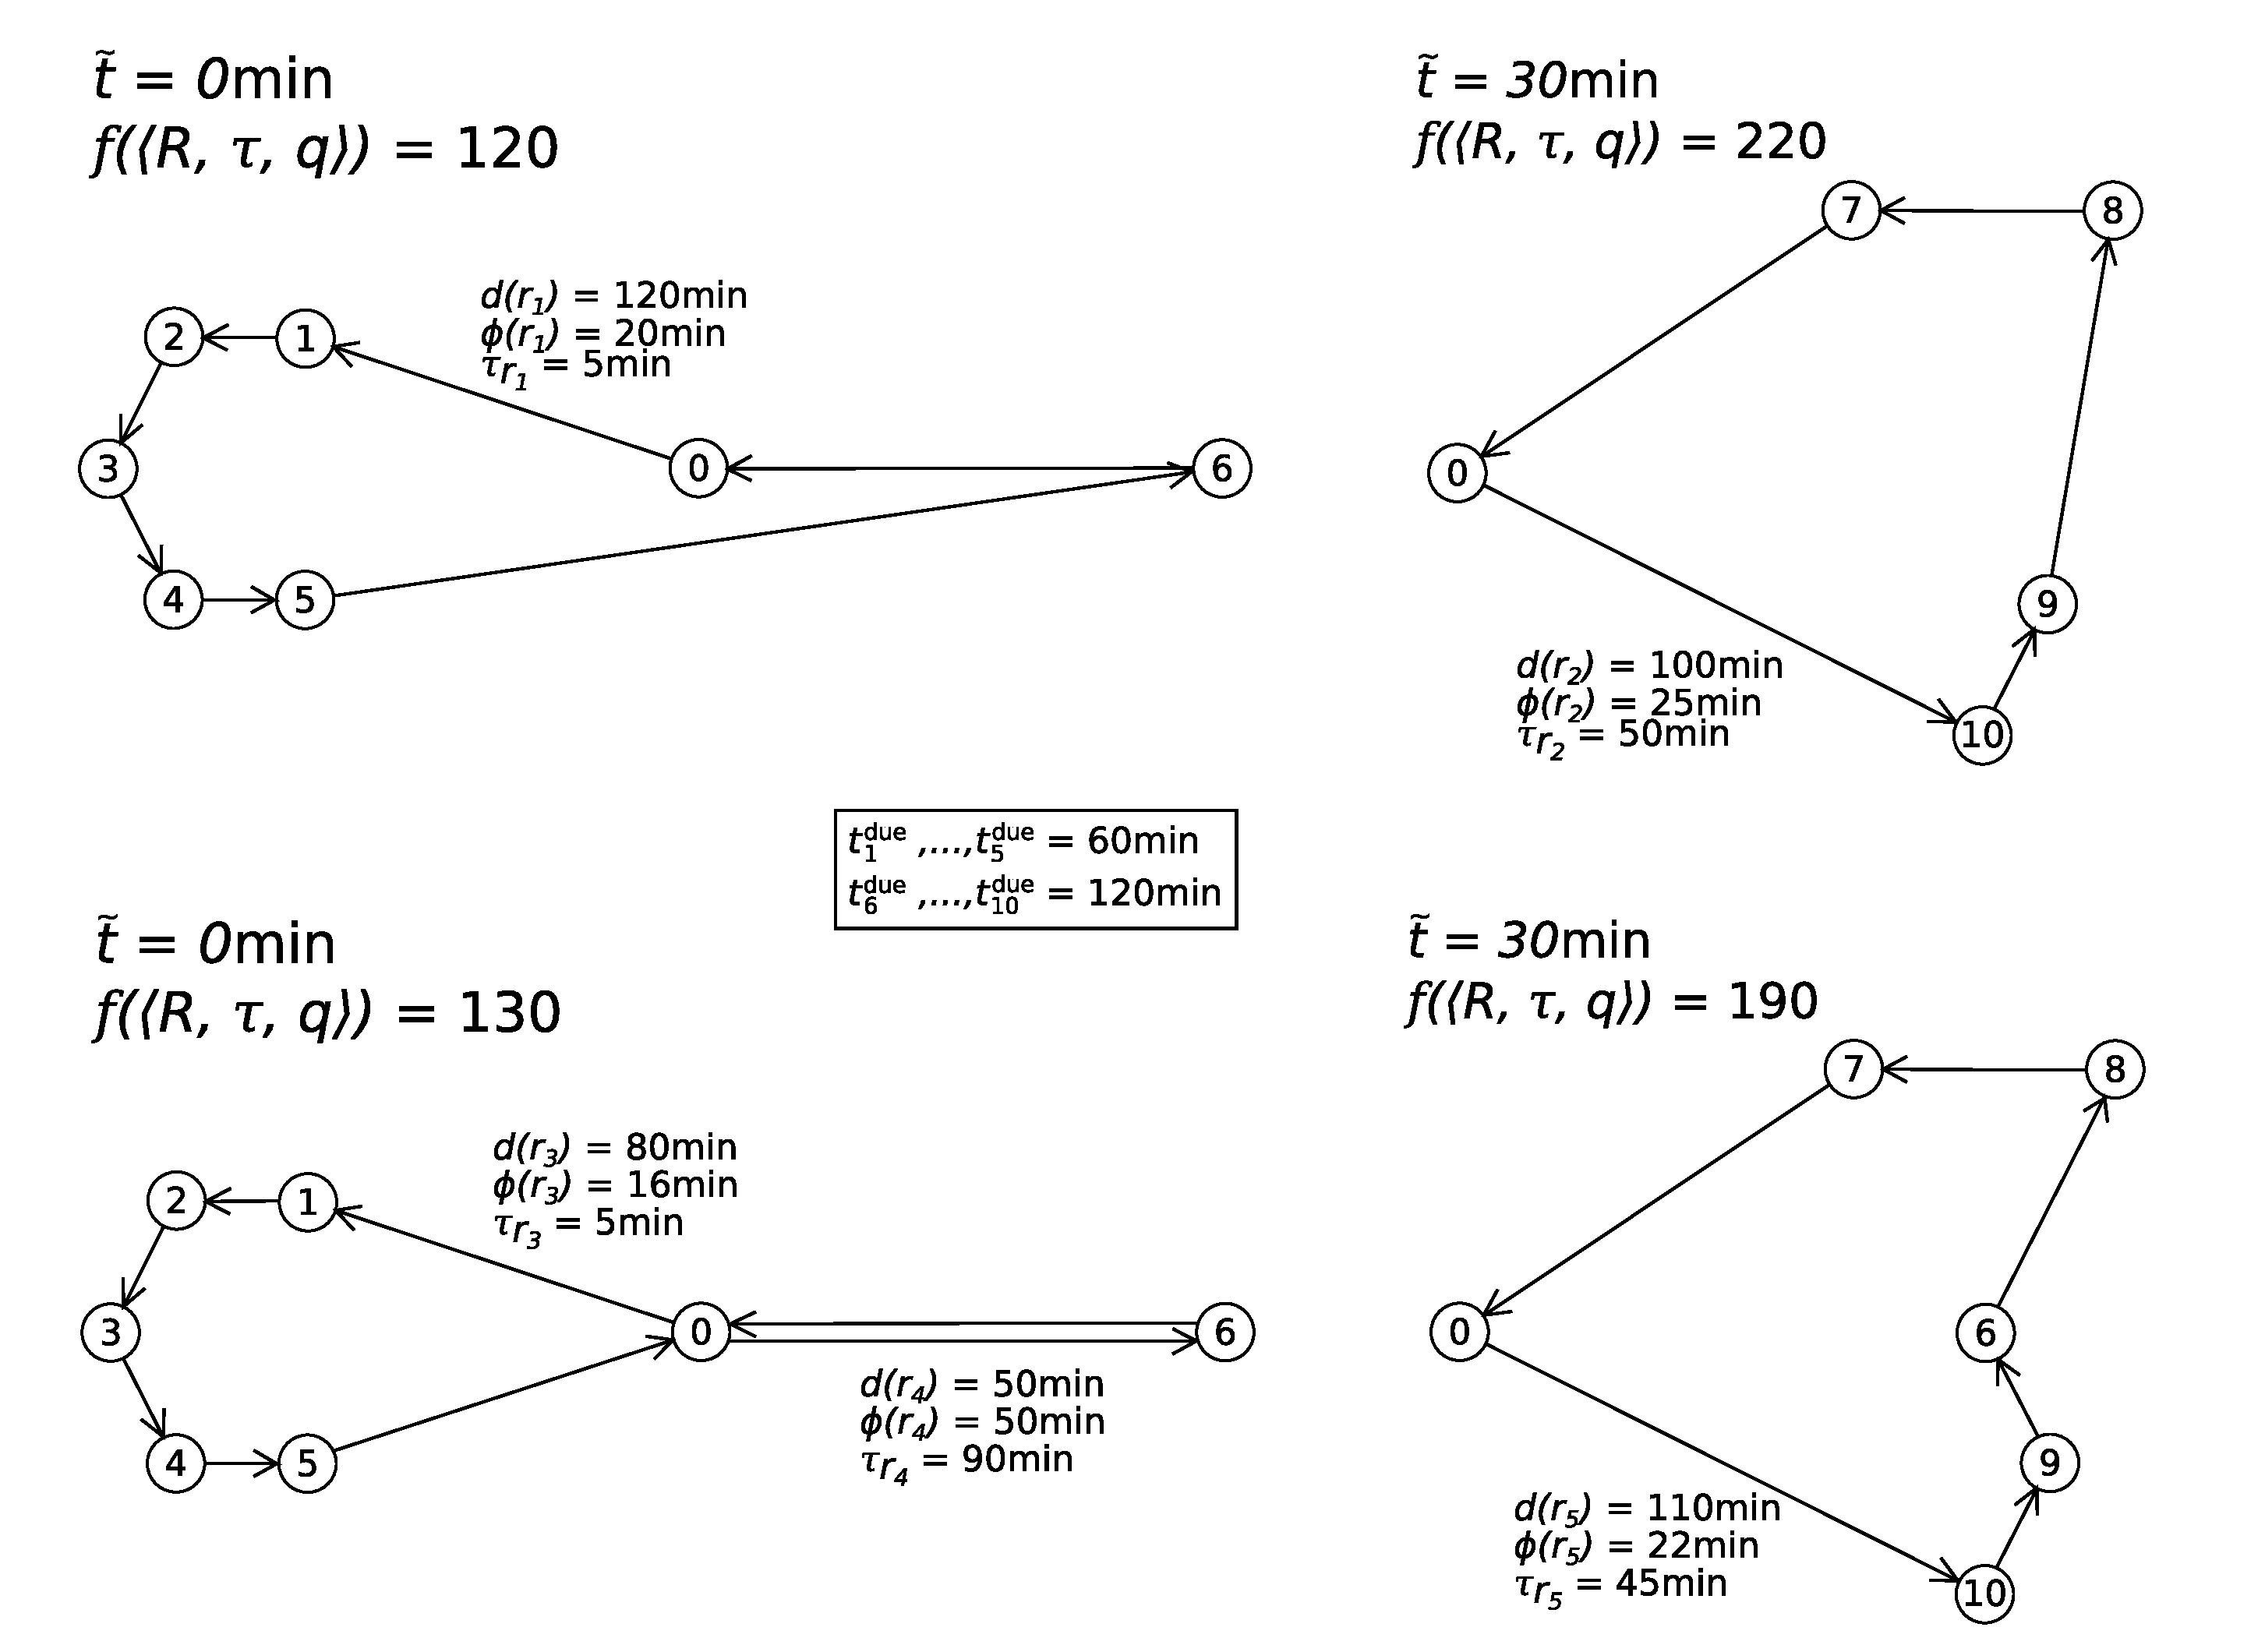
\includegraphics[width=.80\columnwidth]{graphics/illustrative_example_corrected.pdf}
		%\caption{Taken from Bracher et al.~(2021), p.~7}
	\end{figure}
\end{frame}



\begin{frame}{Classical Approach to Consider Future: Scenario Sampling}

See, e.g., \cite{voccia2019same}, \cite{Bent2004}, \cite{Hvattum2006}

\bigskip
\begin{itemize}
	\itemsep2ex
	\item \important{Sample scenario instances} containing artificial future orders\\ according to an expected distribution
	\item \important{Solve} each scenario
	\item Combine solutions to a single \important{consensus solution} for actually available orders
	\item[$\rightarrow$] usually \important{much better}, but \alert{computationally expensive}
\end{itemize}
\end{frame}


\begin{frame}
	\frametitle{Learning a Surrogate Evaluation Function}
	
	{\small\color{gray}\cite{bracher-21}}
	%\textbf{Issue:} depot returns not anticipated
	
	% \begin{itemize}
	% 	\item static LNS happily \alert{mixes urgent and non-urgent orders}
	% 	\item focuses on the geographical aspect, when deadlines are met
	% \end{itemize}	
	\vfill
	
	%\pause
	\structure{Evaluation of routes within LNS:}
	\bigskip
	\begin{itemize}
		\itemsep2ex
		\item replace route duration $d(r)$ by parameterized \important{surrogate travel time} $d'(r)$
		\item predicts an expected \important{discouted travel time} considering that future orders may be combined with current orders in a route
		\item \important{supervised learning} in an \important{offline} phase using \important{scenario sampling}
		\item resulting surrogate directly used in online LNS optimization
	\end{itemize}
	\bigskip
\end{frame}

\begin{frame}{Mean Order Delivery Time / Driver Performance}% \\ \small \textcolor{gray}{Beardwood et al. (1959), Daganzo (1984), Figliozzi (2008, 2010)}}
	Given a day $a$ and an hour $t$, we define the \important{mean order delivery time} $\phi_t(a)$, the time needed by an average driver to deliver one order.
	\bigskip

	\begin{figure}[tb]
		\centering
		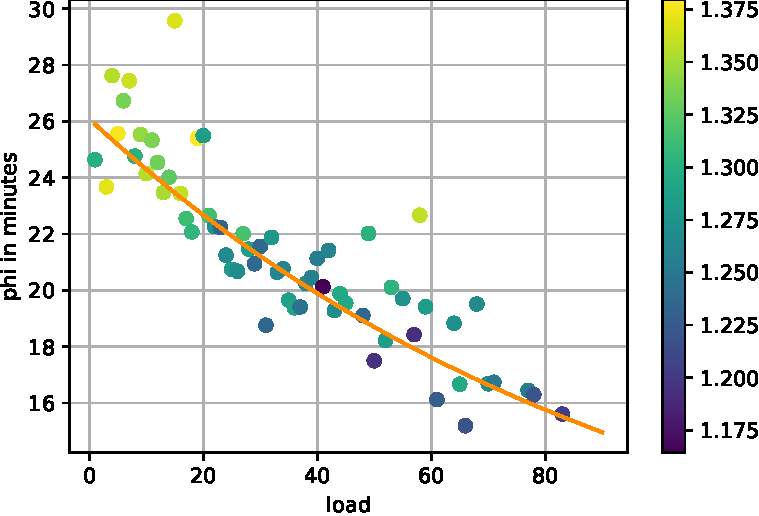
\includegraphics[width=.80\columnwidth]{graphics/phi_fit}
	\end{figure}
\end{frame}

\begin{frame}
	\frametitle{Discounted Route Duration with ML Model $g_\Theta$}
	\begin{equation}
		d'(r) = \begin{cases}
			g_\Theta (d(r), l_r, \omega(\tilde t, \tau_r),\hat\phi,\ldots) & \mbox{ if } \tau_r>\tilde t \land \phi(r)>\hat\phi \\
			d(r) & \mbox{ else}.
		\end{cases}
		\label{eq:d_prime}
	\end{equation}

	\bigskip
	\structure{Parameters / features:}
	\medskip
	\begin{itemize}
		\itemsep1ex
		\item {Route duration:} $d(r)$
		\item {Number of orders in route:} $l_r$
		\item {Current time:} $\tilde t$
		\item {Latest departure time of route:} $\tau_r$
		\item {How many orders to expect before route is started:} $\omega(\tilde t, \tau_r)$
		\item {Expected average time per order:} $\hat \phi$
		\item {Further features derived from the above}
	\end{itemize}
\end{frame}

\begin{frame}
	\frametitle{Considered Models for $g_\Theta$}
	\begin{itemize}
		\itemsep2ex
		\item \important{Exponential function}: (educated guess) 
		\begin{equation*}
				g^\mathrm{exp}_\rho(d(r), l_r, \omega(\tilde t, \tau_r), \hat\phi) = d(r) - (d(r)-\hat\phi \cdot l_r) \cdot (1-e^{-\rho \cdot \omega(\tilde t, \tau_r)})
		\end{equation*}
		\vspace{-7mm}
		\begin{figure}[tb]
			\centering
			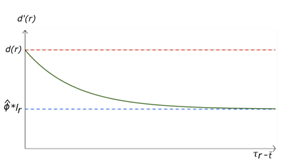
\includegraphics[width=.550\columnwidth]{graphics/exp-model.png}
		\end{figure}
		just parameter $\rho$ has to be learned
		\item \important{Linear regression}
		\item \important{Multilayer perceptron}\\
		fully connected, two hidden layers, ReLU activation function
	\end{itemize}
\end{frame}


\begin{frame}
	\frametitle{Results}
	\centering
	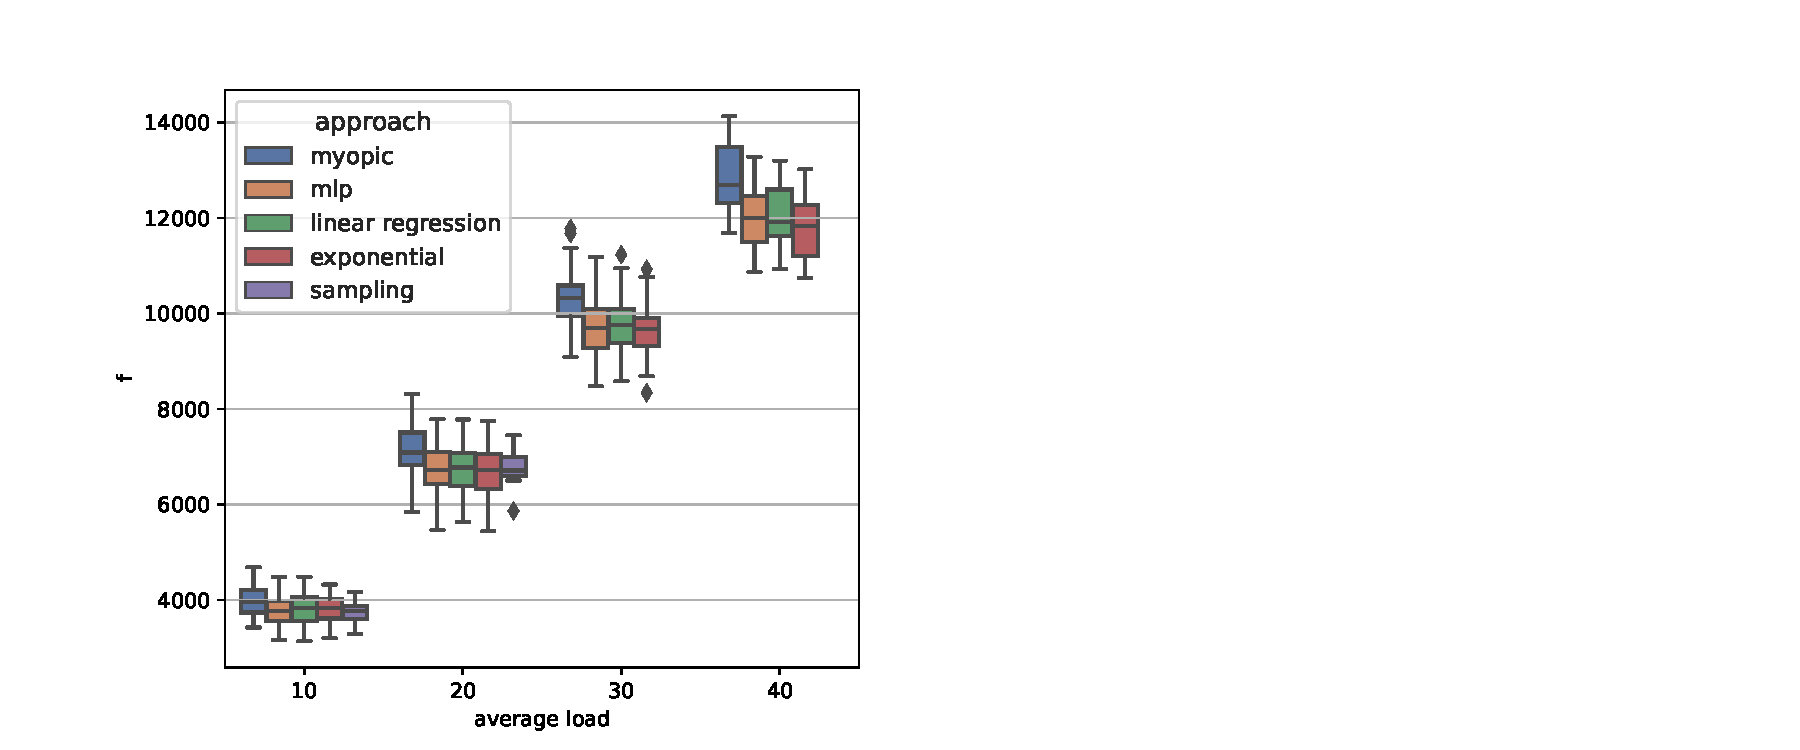
\includegraphics[width=0.7\textwidth]{graphics/boxplots.pdf}
\end{frame}


\begin{frame}
	\frametitle{Conclusions to Dynamic Problem}
	
	\begin{itemize}
		\itemsep2ex
		%\item \important{Dynamic Stochastic VRPs} are challenging
		\item $\approx$5--10\% improvement in travel times with 30-40 orders
		\item Described approach uses the power of the state-of-the-art for the static problem
		\item \important{Scenario Sampling} can be precise, but often too computationally expensive
		\item Learned \important{surrogate models} can be highly effective and are faster
		\item \important{More complex models are not necessarily better!}
	\end{itemize}
\end{frame}
	

\end{document}



	
	
% \begin{frame}
% 	%\frametitle{Discussion \& Questions}
% 	\centering
% 	\huge 
% 	Thank you!
	
% %	\bigskip
% %	
% %	Questions?

% \end{frame}





% ### Additional Slides ############################################

\begin{frame}[noframenumbering]
	\frametitle{Typical DARP Features \footnotesize{\textcolor{gray}{\cite{Ho:2018}}}}

\begin{itemize}
	\item \textbf{Request:} transportation from a pickup to a drop-off location
	\item \textbf{Time window:} earliest and latest times of pickup/drop-off %for a request
	%\item Vehicle(s): ?
%	\item \textbf{Depot(s):} starting and ending location(s) of a trip of a vehicle
%	\item \textbf{Route (trip):} a vehicle's tour starting and ending at a depot
	\item \textbf{Route:} a vehicle's tour % starting and ending at a depot
	\item \textbf{Depot(s):} starting and ending location(s) of a route 
	\item \textbf{Vehicle capacity:} maximum number of users in a vehicle at once
	\item \textbf{Load:} number of users in a vehicle
	\item \textbf{(Maximum) Ride time:} (maximum) time a user spends in a vehicle
%	\item \textbf{Waiting time:} time without service or travel
	\item \textbf{(Maximum) Route duration:} (maximum) travel time of a vehicle for one tour
\end{itemize}
	
\end{frame}

\begin{frame}[noframenumbering]
	\frametitle{Routing and Scheduling in E-ADARP \\ \footnotesize{\textcolor{gray}{\cite{Cordeau:2007,Bongiovanni:2019}}}}
	
\structure{Routing:} %determine
\begin{itemize}
	\item Sequence of pickup and drop-off locations
	\item Visits to charging stations 
\end{itemize} 

\bigskip

\structure{Scheduling:} %determine 
\begin{itemize}
	\item Departure time from the depot 
	\item Service start time at each location 
	\item Time for (partial) recharging 
\end{itemize}

\bigskip

\structure{Goals:} %(done) remove goals?
\begin{itemize}
%	\item Serve all requests % -> not relevant for a single route 
	\item Satisfy constraints 
	\item Minimize route duration and user excess ride time 
\end{itemize}
	
\end{frame}

\begin{frame}[noframenumbering]
%  \frametitle{Preprocessing {\footnotesize{\textcolor{gray}{(\cite{Dumas:1991, Cordeau:2006})}}}}
  \frametitle{Preprocessing}
  
\structure{Goal:} reduce the size of problem instances

\bigskip

\structure{Time Window Tightening:} {\footnotesize{\textcolor{gray}{\cite{Su:2023}}}}
\smallskip
\begin{itemize}
	\item Tighten known time windows
	\item Determine missing time windows  
\end{itemize}

\bigskip

\structure{Arc Elimination:} {\footnotesize{\textcolor{gray}{\cite{Goeke:2019,Dumas:1991,Cordeau:2006}}}} % remove infeasible arcs based on 
\smallskip
\begin{itemize}
	\item Remove infeasible arcs based on constraints 
%	\item pairing and precedence constraints 
%	\item time windows 
%	\item maximum user ride time 
%	\item battery constraints 
%	\item capacity constraints 
	\item Identify incompatible user pairs 
		\begin{itemize}
			\item[$\rightarrow$] forbid assignment to the same vehicle 
		\end{itemize}
\end{itemize}

%\medskip
%
%\structure{Variable Fixing / Incompatibility Identification:} 
%\begin{itemize}
%	\item use knowledge of infeasible arcs to determine incompatible user pairs 
%	\item forbid assignment of incompatible users to the same vehicle 
%\end{itemize}

\end{frame}

\begin{frame}[noframenumbering]
  \frametitle{Large Neighborhood Search (LNS)}
  \framesubtitle{Initial Solution Construction}
  
\structure{Step 1:} 
\begin{itemize}
	\item Initialize an empty route for each vehicle % {\footnotesize{\textcolor{gray}{(similar to \cite{Bongiovanni:2022})}}}
		\begin{itemize}
			\item Start = predefined origin depot 
			\item End = nearest unvisited destination depot
		\end{itemize}
\end{itemize}

\bigskip

\structure{Step 2:} insert requests 
\begin{itemize}
	\item Time window order based repair operator
\end{itemize}

\bigskip

\structure{Result:} valid solution satisfying all constraints 
\begin{itemize}
	%\item valid solution satisfying all constraints 
	\item Unserved requests possible
\end{itemize}

\end{frame}

\begin{frame}[noframenumbering]
	\frametitle{On-The-Fly Charging Stop Insertion}
	\framesubtitle{MILP I}
	
Inputs:
\begin{itemize}
	\item $d_i$ = service duration at location at index $i$ ($i$-th stop)
	\item $t_{i, j}$ = travel time from $i$-th to $j$-th stop %location at index $i$ to location at index $j$
	\item $[w^{\mathrm{start}}_i, w^{\mathrm{stop}}_i]$ = time window of $i$-th stop %location at index $i$ 
	\item $b_i$ = battery consumption of $i$-th stop 
	\item $Q$ = battery capacity of vehicle 
	\item $\alpha_s$ = charging rate of station $s$
	\item $\beta_{i,j}$ = battery consumption of arc between $i$-th and $j$-th stop %location at index $i$ and location at index $j$
%	\item $u_i$ = maximum ride time of user $i$
\end{itemize}

Decision variables:
\begin{itemize}
	\item $x_{i, s}$ = 1 if charging station $s$ is visited directly before $i$-th stop, 0 otherwise
	\item $d^\mathrm{ch}_{i,s}$ = charging duration at station $s$ before $i$-th stop 
	\item $t^\mathrm{serv}_i$ = service start time at $i$-th stop %location at index $i$ 
	\item $B_i$ = battery level on arrival at the $i$-th stop
	\item $B_i^\mathrm{ch}$ = battery level on arrival at charging station before $i$-th stop
\end{itemize}
	
\end{frame}

\begin{frame}[noframenumbering]
	\frametitle{On-The-Fly Charging Stop Insertion}
	\framesubtitle{MILP II}
	
%{\footnotesize\allowdisplaybreaks
%{\footnotesize
\resizebox{\columnwidth}{!}{
\begin{minipage}{\linewidth}
\small
\begin{align}
	\label{eq:milp-otf_objective-function} \min\quad& \sum_{i=2}^{|R|} \sum_{s\in S} (t_{i-1,s}+t_{s,i}-t_{i-1,i})\cdot x_{i,s} \\
	\label{eq:milp-otf_only-one-xis-per-i} \text{s.t.}\quad & \sum_{s\in S} x_{i,s} \le 1 & i=2,\ldots,|R| \\
	\label{eq:milp-otf_service-times}& t^\mathrm{serv}_i \ge t^\mathrm{serv}_{i-1} + d_{i-1} + t_{i-1,i} + \sum_{s\in S}\left((t_{i-1,s}+t_{s,i}-t_{i-1,i})\cdot x_{i,s} + d^\mathrm{ch}_{i,s}\right) \hspace*{-25mm} & \nonumber\\
	& & i=2,\ldots,|R| \\
	\label{eq:milp-otf_battery-levels_stations}& B_i^\mathrm{ch} = B_{i-1} - \sum_{s\in S}\beta_{i-1,s}x_{i,s} & i=2,\dots,|R| \\
	\label{eq:milp-otf_battery-levels_charging-capacity}& B^\mathrm{ch}_i + \sum_{s\in S}\alpha_s d^\mathrm{ch}_{i,s} \le Q & i=2,\ldots,|R| \\
	\label{eq:milp-otf_battery-levels_stops}& B_i = B^\mathrm{ch}_i + \sum_{s\in S}\alpha_s d^\mathrm{ch}_{i,s} - \beta_{i-1,i} - \sum_{s\in S}(\beta_{s,i}-\beta_{i-1,i})\cdot x_{i,s} - b_i \hspace*{-20mm} & \nonumber \\
	& & i=2,\dots,|R| 
\end{align}
\end{minipage}
}

%\label{eq:milp-otf_charging-duration_upper-bound}& d^\mathrm{ch}_{i,s} \le \frac{Q}{\alpha_s}x_{i,s} & i=2,\ldots,|R|,\ s\in S \\
%	\label{eq:milp-otf_domain_xis}& x_{i,s} \in \{0,1\} & i=2,\ldots,|R|,\ s\in S\\
%	\label{eq:milp-otf_charging-duration_lower_bound}& d^\mathrm{ch}_{i,s} \ge 0 & i=2,\ldots,|R|,\ s\in S\\
%	\label{eq:milp-otf_bounds_battery-levels-stops}& 0 \le B_i \le Q &  i=2,\ldots,|R|\\
%	\label{eq:milp-otf_bounds_battery-levels-stations}& 0 \le B^\mathrm{ch}_i \le Q &  i=2,\ldots,|R|\\
%	\label{eq:milp-otf_bounds_service-start-times}& w^{\mathrm{start}}_i \leq t^\mathrm{serv}_i \leq w^{\mathrm{stop}}_i & i=1,\ldots,|R|
	
\end{frame}

\begin{frame}[noframenumbering]
	\frametitle{On-The-Fly Charging Stop Insertion}
	\framesubtitle{MILP III}
	
%{\footnotesize\allowdisplaybreaks
%{\footnotesize
\resizebox{\columnwidth}{!}{
\begin{minipage}{\linewidth}
%\footnotesize
\begin{align}
	\label{eq:milp-otf_charging-duration_upper-bound}& d^\mathrm{ch}_{i,s} \le \frac{Q}{\alpha_s}x_{i,s} & i=2,\ldots,|R|,\ s\in S \\
	\label{eq:milp-otf_domain_xis}& x_{i,s} \in \{0,1\} & i=2,\ldots,|R|,\ s\in S\\
	\label{eq:milp-otf_charging-duration_lower_bound}& d^\mathrm{ch}_{i,s} \ge 0 & i=2,\ldots,|R|,\ s\in S\\
	\label{eq:milp-otf_bounds_battery-levels-stops}& 0 \le B_i \le Q &  i=2,\ldots,|R|\\
	\label{eq:milp-otf_bounds_battery-levels-stations}& 0 \le B^\mathrm{ch}_i \le Q &  i=2,\ldots,|R|\\
	\label{eq:milp-otf_bounds_service-start-times}& w^{\mathrm{start}}_i \leq t^\mathrm{serv}_i \leq w^{\mathrm{stop}}_i & i=1,\ldots,|R|
\end{align}
\end{minipage}
}

\end{frame}


\begin{frame}[noframenumbering]
	\frametitle{On-The-Fly Charging Stop Insertion}
	\framesubtitle{Time-Efficient Heuristic}
	
\resizebox{0.55\columnwidth}{!}{
%\scalebox{.7}{
% pseudo code for evluation with otf insertion 
\begin{algorithm}[H] 
%	\footnotesize
%	\scriptsize
	\SetAlgoSkip{}
	\SetArgSty{textnormal}	% prints termination criterion in normal text instead of italics
	\SetKwFunction{FMain}{OTF-Insertion}
	\SetKwProg{Fn}{Procedure}{:}{end}
	\SetKw{And}{ and }
	\SetKw{Or}{ or }
%	\KwIn{candidate route $r$}
	\KwIn{route $r$}
 	\KwOut{feasibility status of $r$}
%	\Fn{\FMain{}}{ % prints "OTF-Insertion():"
  		%\Begin{
  			$r \gets$ remove\_charging\_stops($r$)\;
  			$R \gets$ get\_fragments\_and\_depots($r$)\;
%  			\If{$R \text{ is empty}$}{ % case: infeasible fragment
			\If{contains\_infeasible\_fragment($R$)}{
  				\Return{false\;}
  			}
  			$i^{\mathrm{ch}} \gets none,\ S' \gets$ available\_stations($S$)\;
  			$t^{\mathrm{early}},\ d^{\mathrm{wait}},\ B,\ i^{\mathrm{ch}} \gets$ forward\_pass($R$)\;
  			$t^{\mathrm{late}},\ d^{\mathrm{wait\_back}} \gets$ backward\_pass($R$)\;
  			\If{violates\_time\_windows($t^{\mathrm{early}}$) \Or violates\_time\_windows($t^{\mathrm{late}}$)}{
  				\Return{false\;}
  			}
  			\While{$i^{\mathrm{ch}} \not= none$}{
  				$min\_detour \gets \infty ,\, max\_energy \gets 0 ,\, \hat{i} \gets none$\;
  				\For{$i \text{ in } i^{\mathrm{ch}},\ldots,2,\ s \in S'$}{
  					$\mathit{feasible},\ detour,\ energy \gets$ check\_stop($R, i, s$)\;
  					\If{$\mathit{feasible}$ \And better\_stop($detour, energy, min\_detour, max\_energy$)}{
						$min\_detour \gets detour ,\, max\_energy \gets energy$\;
						$\hat{i} \gets i ,\, \hat{s} \gets s$\;
  					}
  				}
  				\If{$\hat{i} = none$}{
  					\Return{false\;}
  				}
  				insert\_charging\_stop($r, R, \hat{i}, \hat{s}$)\;
%  				\If{is\_battery\_feasible($r$)}{ 
%  					%(done) leave if-statement out? is implemented bc. it allows early termination before variable update but would also be caught by while-condition after update
%					%GR: Yes, I think we can omit it then and save a little space.
%  					\Return{true\;}
%  				}
  				update($t^{\mathrm{early}}, d^{\mathrm{wait}}, t^{\mathrm{late}},d^{\mathrm{wait\_back}}, B, i^{\mathrm{ch}}, S'$)\;
  			}
  			\Return{true\;}
%  \caption{Route evaluation with on-the-fly charging stop insertion.}
  \caption{OTF charging stop insertion and evaluation.}
  \label{alg:otf-insertion} % \label has to be placed AFTER \caption to produce correct cross-references.
\end{algorithm}
}
	
\end{frame}


\begin{frame}[noframenumbering]
  \frametitle{Results}
  
Cordeau instances with $\gamma = 0.4$

% Please add the following required packages to your document preamble:
% \usepackage{multirow}
% \usepackage{graphicx}
% \usepackage[table,xcdraw]{xcolor}
% Beamer presentation requires \usepackage{colortbl} instead of \usepackage[table,xcdraw]{xcolor}
\begin{table}[]
\centering
%\caption{Results on Cordeau instances with $\gamma = 0.4$ for limited CS visits ($n_\mathrm{s} = 1$) and unlimited CS visits ($n_\mathrm{s} = \infty$).  }
\label{tab:eurocast24_results_cordeau_g04}
\resizebox{\columnwidth}{!}{%
\begin{tabular}{lrrrrrrrrrrrrrrrr}
\hline
\multicolumn{1}{c}{}                           & \multicolumn{2}{c}{\begin{tabular}[c]{@{}c@{}}e-ADARP2\end{tabular}} & \multicolumn{3}{c}{\begin{tabular}[c]{@{}c@{}}DA\end{tabular}}                                                                 & \multicolumn{3}{c}{\begin{tabular}[c]{@{}c@{}}BI-LNS\end{tabular}}  & \multicolumn{4}{c}{\begin{tabular}[c]{@{}c@{}}OTF MILP\end{tabular}}               & \multicolumn{4}{c}{\begin{tabular}[c]{@{}c@{}}OTF Heuristic\end{tabular}} \\ \cline{2-17} 
\multicolumn{1}{c}{\multirow{-2}{*}{Instance}} & \begin{tabular}[c]{@{}r@{}}RT \\ {[}min{]}\end{tabular} & \multicolumn{1}{r|}{Obj}             & \begin{tabular}[c]{@{}r@{}}RT mean \\ {[}min{]}\end{tabular} & Obj min         & \multicolumn{1}{r|}{Obj mean}                               & Obj min         & Obj mean                               & \multicolumn{1}{r|}{Feas}  & Obj min         & Obj mean                               & Obj sd & \multicolumn{1}{r|}{Feas}  & Obj min            & Obj mean                                  & Obj sd    & Feas    \\ \hline
\multicolumn{17}{c}{$n_\mathrm{s} = 1$}                                                                                                                                                                                                                                                                                                                                                                                                                                                                                                                                        \\ \hline
a2-16                                          & 0.03                                                    & \multicolumn{1}{r|}{\textbf{237.38}} & 0.88                                                         & \textbf{237.38} & \multicolumn{1}{r|}{{\color[HTML]{FE0000} \textbf{237.38}}} & 238.20          & 238.20                                 & \multicolumn{1}{r|}{10/10} & \textbf{237.38} & {\color[HTML]{FE0000} \textbf{237.38}} & 0.00   & \multicolumn{1}{r|}{30/30} & \textbf{237.38}    & {\color[HTML]{FE0000} \textbf{237.38}}    & 0.00      & 30/30   \\
a2-20                                          & 0.83                                                    & \multicolumn{1}{r|}{\textbf{280.70}} & 2.35                                                         & \textbf{280.70} & \multicolumn{1}{r|}{{\color[HTML]{FE0000} \textbf{280.70}}} & 282.90          & 283.24                                 & \multicolumn{1}{r|}{10/10} & \textbf{280.70} & {\color[HTML]{FE0000} \textbf{280.70}} & 0.00   & \multicolumn{1}{r|}{30/30} & \textbf{280.70}    & {\color[HTML]{FE0000} \textbf{280.70}}    & 0.00      & 30/30   \\
a2-24                                          & 0.42                                                    & \multicolumn{1}{r|}{348.04}          & 3.85                                                         & \textbf{347.04} & \multicolumn{1}{r|}{{\color[HTML]{FE0000} \textbf{347.04}}} & \textbf{347.04} & 349.67                                 & \multicolumn{1}{r|}{10/10} & \textbf{347.04} & 348.14                                 & 1.12   & \multicolumn{1}{r|}{30/30} & 349.20             & 349.20                                    & 0.00      & 30/30   \\
a3-18                                          & 0.07                                                    & \multicolumn{1}{r|}{236.82}          & 0.44                                                         & 236.82          & \multicolumn{1}{r|}{236.82}                                 & 238.73          & 238.73                                 & \multicolumn{1}{r|}{10/10} & \textbf{236.81} & 236.94                                 & 0.43   & \multicolumn{1}{r|}{30/30} & \textbf{236.81}    & {\color[HTML]{FE0000} \textbf{236.81}}    & 0.00      & 30/30   \\
a3-24                                          & 0.28                                                    & \multicolumn{1}{r|}{\textbf{274.80}} & 1.13                                                         & \textbf{274.80} & \multicolumn{1}{r|}{{\color[HTML]{FE0000} \textbf{274.80}}} & 275.58          & 275.58                                 & \multicolumn{1}{r|}{10/10} & \textbf{274.80} & 276.42                                 & 1.34   & \multicolumn{1}{r|}{30/30} & \textbf{274.80}    & {\color[HTML]{FE0000} \textbf{274.80}}    & 0.00      & 30/30   \\
a3-30                                          & 1.65                                                    & \multicolumn{1}{r|}{413.37}          & 1.48                                                         & \textbf{413.34} & \multicolumn{1}{r|}{{\color[HTML]{FE0000} \textbf{413.34}}} & 415.51          & 415.75                                 & \multicolumn{1}{r|}{10/10} & \textbf{413.34} & 415.36                                 & 2.46   & \multicolumn{1}{r|}{30/30} & 413.37             & 413.37                                    & 0.00      & 30/30   \\
a3-36                                          & 5.11                                                    & \multicolumn{1}{r|}{484.14}          & 2.63                                                         & \textbf{483.06} & \multicolumn{1}{r|}{{\color[HTML]{FE0000} \textbf{483.86}}} & 485.98          & 487.42                                 & \multicolumn{1}{r|}{10/10} & \textbf{483.06} & 490.65                                 & 5.00   & \multicolumn{1}{r|}{30/30} & \textbf{483.06}    & 485.92                                    & 2.78      & 30/30   \\
a4-16                                          & 0.09                                                    & \multicolumn{1}{r|}{\textbf{222.49}} & 0.32                                                         & \textbf{222.49} & \multicolumn{1}{r|}{{\color[HTML]{FE0000} \textbf{222.49}}} & \textbf{222.49} & {\color[HTML]{FE0000} \textbf{222.49}} & \multicolumn{1}{r|}{10/10} & \textbf{222.49} & 222.91                                 & 0.46   & \multicolumn{1}{r|}{30/30} & \textbf{222.49}    & {\color[HTML]{FE0000} \textbf{222.49}}    & 0.00      & 30/30   \\
a4-24                                          & 0.66                                                    & \multicolumn{1}{r|}{\textbf{311.03}} & 0.53                                                         & \textbf{311.03} & \multicolumn{1}{r|}{311.65}                                 & 311.48          & 311.48                                 & \multicolumn{1}{r|}{10/10} & \textbf{311.03} & 311.35                                 & 0.30   & \multicolumn{1}{r|}{30/30} & \textbf{311.03}    & {\color[HTML]{FE0000} \textbf{311.03}}    & 0.00      & 30/30   \\
a4-32                                          & 11.36                                                   & \multicolumn{1}{r|}{\textbf{394.26}} & 1.05                                                         & \textbf{394.26} & \multicolumn{1}{r|}{397.21}                                 & 394.96          & 395.45                                 & \multicolumn{1}{r|}{10/10} & \textbf{394.26} & 395.12                                 & 1.10   & \multicolumn{1}{r|}{30/30} & \textbf{394.26}    & {\color[HTML]{FE0000} \textbf{394.26}}    & 0.00      & 30/30   \\
a4-40                                          & 6.96                                                    & \multicolumn{1}{r|}{\textbf{453.84}} & 1.94                                                         & \textbf{453.84} & \multicolumn{1}{r|}{459.46}                                 & 457.01          & 457.39                                 & \multicolumn{1}{r|}{10/10} & \textbf{453.84} & 462.97                                 & 4.77   & \multicolumn{1}{r|}{30/30} & \textbf{453.84}    & {\color[HTML]{FE0000} \textbf{454.84}}    & 1.87      & 30/30   \\
a4-48                                          & 120.00                                                  & \multicolumn{1}{r|}{\textbf{554.60}} & 2.96                                                         & 558.11          & \multicolumn{1}{r|}{563.47}                                 & 557.56          & 560.09                                 & \multicolumn{1}{r|}{10/10} & 556.83          & 563.07                                 & 2.89   & \multicolumn{1}{r|}{30/30} & \textbf{554.60}    & {\color[HTML]{FE0000} \textbf{556.98}}    & 1.49      & 30/30   \\
a5-40                                          & 20.35                                                   & \multicolumn{1}{r|}{414.51}          & 1.21                                                         & 416.25          & \multicolumn{1}{r|}{420.32}                                 & 415.63          & 415.63                                 & \multicolumn{1}{r|}{10/10} & 415.79          & 421.75                                 & 3.91   & \multicolumn{1}{r|}{30/30} & \textbf{414.50}    & {\color[HTML]{FE0000} \textbf{415.12}}    & 1.05      & 30/30   \\
a5-50                                          & 120.00                                                  & \multicolumn{1}{r|}{560.50}          & 2.71                                                         & 567.54          & \multicolumn{1}{r|}{574.56}                                 & 560.41          & {\color[HTML]{FE0000} \textbf{562.55}} & \multicolumn{1}{r|}{10/10} & 566.50          & 576.18                                 & 4.69   & \multicolumn{1}{r|}{30/30} & \textbf{559.51}    & 564.41                                    & 3.44      & 30/30   \\ \hline
\multicolumn{17}{c}{$n_\mathrm{s} = \infty$}                                                                                                                                                                                                                                                                                                                                                                                                                                                                                                                                   \\ \hline
a2-16                                          &                                                         & \multicolumn{1}{r|}{}                & 0.84                                                         & \textbf{237.38} & \multicolumn{1}{r|}{{\color[HTML]{FE0000} \textbf{237.38}}} & 238.20          & 238.20                                 & \multicolumn{1}{r|}{10/10} & \textbf{237.38} & {\color[HTML]{FE0000} \textbf{237.38}} & 0.00   & \multicolumn{1}{r|}{30/30} & \textbf{237.38}    & {\color[HTML]{FE0000} \textbf{237.38}}    & 0.00      & 30/30   \\
a2-20                                          &                                                         & \multicolumn{1}{r|}{}                & 2.42                                                         & 280.70          & \multicolumn{1}{r|}{280.70}                                 & 282.62          & 283.10                                 & \multicolumn{1}{r|}{10/10} & \textbf{280.58} & {\color[HTML]{FE0000} \textbf{280.58}} & 0.21   & \multicolumn{1}{r|}{30/30} & 280.70             & 280.70                                    & 0.00      & 30/30   \\
a2-24                                          &                                                         & \multicolumn{1}{r|}{}                & 4.43                                                         & \textbf{346.28} & \multicolumn{1}{r|}{{\color[HTML]{FE0000} \textbf{346.28}}} & 347.93          & 349.07                                 & \multicolumn{1}{r|}{10/10} & \textbf{346.28} & 346.56                                 & 0.05   & \multicolumn{1}{r|}{30/30} & 348.92             & 348.92                                    & 0.00      & 30/30   \\
a3-18                                          &                                                         & \multicolumn{1}{r|}{}                & 0.42                                                         & 236.82          & \multicolumn{1}{r|}{236.82}                                 & 238.73          & 238.73                                 & \multicolumn{1}{r|}{10/10} & \textbf{236.81} & 236.91                                 & 0.76   & \multicolumn{1}{r|}{30/30} & \textbf{236.81}    & {\color[HTML]{FE0000} \textbf{236.81}}    & 0.00      & 30/30   \\
a3-24                                          &                                                         & \multicolumn{1}{r|}{}                & 1.11                                                         & \textbf{274.80} & \multicolumn{1}{r|}{{\color[HTML]{FE0000} \textbf{274.80}}} & 275.18          & 275.46                                 & \multicolumn{1}{r|}{10/10} & \textbf{274.80} & 275.49                                 & 0.96   & \multicolumn{1}{r|}{30/30} & \textbf{274.80}    & {\color[HTML]{FE0000} \textbf{274.80}}    & 0.00      & 30/30   \\
a3-30                                          &                                                         & \multicolumn{1}{r|}{}                & 1.73                                                         & 413.34          & \multicolumn{1}{r|}{{\color[HTML]{FE0000} \textbf{413.34}}} & 415.51          & 415.81                                 & \multicolumn{1}{r|}{10/10} & \textbf{413.28} & 414.51                                 & 1.87   & \multicolumn{1}{r|}{30/30} & 413.37             & 413.37                                    & 0.00      & 30/30   \\
a3-36                                          &                                                         & \multicolumn{1}{r|}{}                & 4.15                                                         & \textbf{481.17} & \multicolumn{1}{r|}{{\color[HTML]{FE0000} \textbf{481.17}}} & 484.07          & 485.37                                 & \multicolumn{1}{r|}{10/10} & \textbf{481.17} & 487.67                                 & 3.64   & \multicolumn{1}{r|}{30/30} & \textbf{481.17}    & 482.68                                    & 2.26      & 30/30   \\
a4-16                                          &                                                         & \multicolumn{1}{r|}{}                & 0.30                                                         & \textbf{222.49} & \multicolumn{1}{r|}{{\color[HTML]{FE0000} \textbf{222.49}}} & \textbf{222.49} & {\color[HTML]{FE0000} \textbf{222.49}} & \multicolumn{1}{r|}{10/10} & \textbf{222.49} & 223.14                                 & 0.54   & \multicolumn{1}{r|}{30/30} & \textbf{222.49}    & {\color[HTML]{FE0000} \textbf{222.49}}    & 0.00      & 30/30   \\
a4-24                                          &                                                         & \multicolumn{1}{r|}{}                & 0.49                                                         & \textbf{311.03} & \multicolumn{1}{r|}{311.65}                                 & 311.48          & 311.48                                 & \multicolumn{1}{r|}{10/10} & \textbf{311.03} & 311.28                                 & 0.47   & \multicolumn{1}{r|}{30/30} & \textbf{311.03}    & {\color[HTML]{FE0000} \textbf{311.03}}    & 0.00      & 30/30   \\
a4-32                                          &                                                         & \multicolumn{1}{r|}{}                & 1.03                                                         & \textbf{394.26} & \multicolumn{1}{r|}{397.27}                                 & 394.96          & 395.15                                 & \multicolumn{1}{r|}{10/10} & \textbf{394.26} & 395.58                                 & 1.19   & \multicolumn{1}{r|}{30/30} & \textbf{394.26}    & {\color[HTML]{FE0000} \textbf{394.26}}    & 0.00      & 30/30   \\
a4-40                                          &                                                         & \multicolumn{1}{r|}{}                & 2.02                                                         & \textbf{453.84} & \multicolumn{1}{r|}{458.74}                                 & 456.93          & 457.50                                 & \multicolumn{1}{r|}{10/10} & 455.22          & 463.28                                 & 3.85   & \multicolumn{1}{r|}{30/30} & \textbf{453.84}    & {\color[HTML]{FE0000} \textbf{454.53}}    & 1.84      & 30/30   \\
a4-48                                          &                                                         & \multicolumn{1}{r|}{}                & 3.86                                                         & 558.96          & \multicolumn{1}{r|}{564.86}                                 & 557.63          & 559.63                                 & \multicolumn{1}{r|}{10/10} & 556.09          & 561.83                                 & 3.26   & \multicolumn{1}{r|}{30/30} & \textbf{555.25}    & {\color[HTML]{FE0000} \textbf{556.40}}    & 1.24      & 30/30   \\
a5-40                                          &                                                         & \multicolumn{1}{r|}{}                & 1.18                                                         & 415.79          & \multicolumn{1}{r|}{419.82}                                 & 415.62          & 415.62                                 & \multicolumn{1}{r|}{10/10} & 416.98          & 423.21                                 & 3.79   & \multicolumn{1}{r|}{30/30} & \textbf{414.50}    & {\color[HTML]{FE0000} \textbf{414.91}}    & 0.82      & 30/30   \\
a5-50                                          &                                                         & \multicolumn{1}{r|}{}                & 3.07                                                         & 567.13          & \multicolumn{1}{r|}{574.28}                                 & 560.41          & {\color[HTML]{FE0000} \textbf{562.64}} & \multicolumn{1}{r|}{10/10} & 562.56          & 574.19                                 & 7.02   & \multicolumn{1}{r|}{30/30} & \textbf{559.48}    & 562.81                                    & 2.78      & 30/30   \\ \hline
\end{tabular}%
}
\end{table}

\end{frame}


\begin{frame}[noframenumbering]
  \frametitle{Results}
  
Ropke instances with $\gamma = 0.4$

%\fixme{MILP has only 29 runs for $n_\mathrm{s} = \infty$} %TODO MILP has only 29 runs for $n_\mathrm{s} = \infty$
% Please add the following required packages to your document preamble:
% \usepackage{multirow}
% \usepackage{graphicx}
% \usepackage[table,xcdraw]{xcolor}
% Beamer presentation requires \usepackage{colortbl} instead of \usepackage[table,xcdraw]{xcolor}
\begin{table}[]
\centering
%\caption{Results on Ropke instances with $\gamma = 0.4$ for limited CS visits ($n_\mathrm{s} = 1$) and unlimited CS visits ($n_\mathrm{s} = \infty$).  }
\label{tab:eurocast24_results_ropke_g04}
\resizebox{\columnwidth}{!}{%
\begin{tabular}{lrrrrrrrrrrrrrr}
\hline
\multicolumn{1}{c}{}                           & \multicolumn{3}{c}{\begin{tabular}[c]{@{}c@{}}DA\end{tabular}}                           & \multicolumn{3}{c}{\begin{tabular}[c]{@{}c@{}}BI-LNS\end{tabular}}  & \multicolumn{4}{c}{\begin{tabular}[c]{@{}c@{}}OTF MILP\end{tabular}} & \multicolumn{4}{c}{\begin{tabular}[c]{@{}c@{}}OTF Heuristic\end{tabular}} \\ \cline{2-15} 
\multicolumn{1}{c}{\multirow{-2}{*}{Instance}} & \begin{tabular}[c]{@{}r@{}}RT mean \\ {[}min{]}\end{tabular} & Obj min & \multicolumn{1}{r|}{Obj mean} & Obj min         & Obj mean                               & \multicolumn{1}{r|}{Feas}  & Obj min       & Obj mean       & Obj sd       & \multicolumn{1}{r|}{Feas}        & Obj min             & Obj mean                                  & Obj sd   & Feas    \\ \hline
\multicolumn{15}{c}{$n_\mathrm{s} = 1$}                                                                                                                                                                                                                                                                                                                                                                                   \\ \hline
a5-60                                          & 4.89                                                         & 697.97  & \multicolumn{1}{r|}{718.44}   & 688.16          & 693.43                                 & \multicolumn{1}{r|}{10/10} & 691.49        & 703.42         & 5.68         & \multicolumn{1}{r|}{30/30}       & \textbf{685.51}     & {\color[HTML]{FE0000} \textbf{690.63}}    & 2.94     & 30/30   \\
a6-48                                          & 4.29                                                         & 506.91  & \multicolumn{1}{r|}{514.46}   & 506.85          & 507.43                                 & \multicolumn{1}{r|}{10/10} & 508.70        & 515.80         & 4.66         & \multicolumn{1}{r|}{30/30}       & \textbf{506.45}     & {\color[HTML]{FE0000} \textbf{506.84}}    & 0.30     & 30/30   \\
a6-60                                          & 2.89                                                         & 694.78  & \multicolumn{1}{r|}{706.07}   & 692.69          & 695.13                                 & \multicolumn{1}{r|}{10/10} & 698.53        & 705.90         & 5.77         & \multicolumn{1}{r|}{30/30}       & \textbf{690.29}     & {\color[HTML]{FE0000} \textbf{693.16}}    & 2.31     & 30/30   \\
a6-72                                          & 5.83                                                         & 799.60  & \multicolumn{1}{r|}{821.17}   & 771.97          & 778.30                                 & \multicolumn{1}{r|}{10/10} & 783.18        & 795.86         & 8.00         & \multicolumn{1}{r|}{30/30}       & \textbf{765.64}     & {\color[HTML]{FE0000} \textbf{776.00}}    & 4.47     & 30/30   \\
a7-56                                          & 1.67                                                         & 613.66  & \multicolumn{1}{r|}{624.40}   & 614.58          & 616.02                                 & \multicolumn{1}{r|}{10/10} & 618.27        & 628.57         & 5.52         & \multicolumn{1}{r|}{30/30}       & \textbf{612.78}     & {\color[HTML]{FE0000} \textbf{615.27}}    & 2.51     & 30/30   \\
a7-70                                          & 4.56                                                         & 766.05  & \multicolumn{1}{r|}{784.54}   & 761.62          & 765.71                                 & \multicolumn{1}{r|}{10/10} & 763.06        & 778.86         & 8.93         & \multicolumn{1}{r|}{30/30}       & \textbf{756.46}     & {\color[HTML]{FE0000} \textbf{760.21}}    & 2.03     & 30/30   \\
a7-84                                          & 9.74                                                         & 932.12  & \multicolumn{1}{r|}{NA}       & 886.19          & 891.04                                 & \multicolumn{1}{r|}{10/10} & 893.14        & 914.92         & 11.51        & \multicolumn{1}{r|}{30/30}       & \textbf{878.99}     & {\color[HTML]{FE0000} \textbf{890.18}}    & 7.23     & 30/30   \\
a8-64                                          & 10.69                                                        & 638.36  & \multicolumn{1}{r|}{652.30}   & 637.95          & 640.41                                 & \multicolumn{1}{r|}{10/10} & 646.28        & 655.15         & 5.41         & \multicolumn{1}{r|}{30/30}       & \textbf{632.95}     & {\color[HTML]{FE0000} \textbf{639.02}}    & 3.05     & 30/30   \\
a8-80                                          & 7.47                                                         & 811.19  & \multicolumn{1}{r|}{833.05}   & \textbf{793.17} & {\color[HTML]{FE0000} \textbf{798.41}} & \multicolumn{1}{r|}{10/10} & 811.62        & 823.98         & 7.00         & \multicolumn{1}{r|}{30/30}       & 794.04              & {\color[HTML]{000000} 800.85}             & 5.13     & 30/30   \\
a8-96                                          & 10.29                                                        & NA      & \multicolumn{1}{r|}{NA}       & 1048.72         & 1057.47                                & \multicolumn{1}{r|}{10/10} & 1055.03       & 1080.91        & 10.41        & \multicolumn{1}{r|}{30/30}       & \textbf{1036.22}    & {\color[HTML]{FE0000} \textbf{1047.47}}   & 5.62     & 30/30   \\ \hline
\multicolumn{15}{c}{$n_\mathrm{s} = \infty$}                                                                                                                                                                                                                                                                                                                                                                              \\ \hline
a5-60                                          & 4.75                                                         & 691.72  & \multicolumn{1}{r|}{709.78}   & 685.68          & 689.42                                 & \multicolumn{1}{r|}{10/10} & 691.64        & 698.91         & 4.29         & \multicolumn{1}{r|}{30/30}       & \textbf{683.85}     & {\color[HTML]{FE0000} \textbf{686.91}}    & 2.53     & 30/30   \\
a6-48                                          & 4.26                                                         & 507.25  & \multicolumn{1}{r|}{514.64}   & 506.85          & 507.30                                 & \multicolumn{1}{r|}{10/10} & 507.82        & 518.25         & 5.12         & \multicolumn{1}{r|}{30/30}       & \textbf{506.45}     & {\color[HTML]{FE0000} \textbf{506.87}}    & 0.22     & 30/30   \\
a6-60                                          & 2.90                                                         & 692.83  & \multicolumn{1}{r|}{701.86}   & 692.25          & {\color[HTML]{FE0000} \textbf{693.68}} & \multicolumn{1}{r|}{10/10} & 698.82        & 705.81         & 4.47         & \multicolumn{1}{r|}{30/30}       & \textbf{690.40}     & {\color[HTML]{000000} 693.72}             & 2.62     & 30/30   \\
a6-72                                          & 5.71                                                         & 781.22  & \multicolumn{1}{r|}{801.86}   & 774.38          & 778.84                                 & \multicolumn{1}{r|}{10/10} & 784.50        & 797.62         & 9.52         & \multicolumn{1}{r|}{30/30}       & \textbf{762.05}     & {\color[HTML]{FE0000} \textbf{772.91}}    & 4.45     & 30/30   \\
a7-56                                          & 1.65                                                         & 615.74  & \multicolumn{1}{r|}{623.51}   & 614.58          & 615.40                                 & \multicolumn{1}{r|}{10/10} & 619.52        & 629.99         & 4.88         & \multicolumn{1}{r|}{30/30}       & \textbf{612.53}     & {\color[HTML]{FE0000} \textbf{614.78}}    & 2.15     & 30/30   \\
a7-70                                          & 4.56                                                         & 761.58  & \multicolumn{1}{r|}{778.04}   & 762.78          & 764.51                                 & \multicolumn{1}{r|}{10/10} & 767.89        & 784.46         & 9.43         & \multicolumn{1}{r|}{30/30}       & \textbf{757.01}     & {\color[HTML]{FE0000} \textbf{760.15}}    & 2.23     & 30/30   \\
a7-84                                          & 7.61                                                         & 896.91  & \multicolumn{1}{r|}{916.23}   & 884.94          & 890.81                                 & \multicolumn{1}{r|}{10/10} & 901.72        & 916.28         & 11.20        & \multicolumn{1}{r|}{30/30}       & \textbf{877.98}     & {\color[HTML]{FE0000} \textbf{886.22}}    & 5.82     & 30/30   \\
a8-64                                          & 11.99                                                        & 637.84  & \multicolumn{1}{r|}{652.17}   & 637.95          & 640.30                                 & \multicolumn{1}{r|}{10/10} & 649.89        & 662.91         & 8.31         & \multicolumn{1}{r|}{29/29}       & \textbf{632.21}     & {\color[HTML]{FE0000} \textbf{639.48}}    & 3.15     & 30/30   \\
a8-80                                          & 7.52                                                         & 813.16  & \multicolumn{1}{r|}{829.92}   & 794.38          & {\color[HTML]{FE0000} \textbf{797.08}} & \multicolumn{1}{r|}{10/10} & 825.43        & 835.17         & 6.71         & \multicolumn{1}{r|}{29/29}       & \textbf{793.39}     & {\color[HTML]{000000} 802.36}             & 5.25     & 30/30   \\
a8-96                                          & 9.41                                                         & 1058.41 & \multicolumn{1}{r|}{1090.04}  & 1048.45         & 1053.35                                & \multicolumn{1}{r|}{10/10} & 1068.79       & 1082.10        & 8.35         & \multicolumn{1}{r|}{29/29}       & \textbf{1034.17}    & {\color[HTML]{FE0000} \textbf{1043.42}}   & 6.12     & 30/30   \\ \hline
\end{tabular}%
}
\end{table}

\end{frame}



\end{document}
